         \chapter{Vectors and scalars}\fancyfoot[LO,RE]{Physics: Mechanics}\label{chap:vectors}
    \setcounter{figure}{1}
    \setcounter{subfigure}{1}
    \label{59e414b70efc194a27a122db47d06ce6}
         \section{Introduction to vectors and scalars}
    \nopagebreak
%            \label{m38812} $ \hspace{-5pt}\begin{array}{cccccccccccc}   
\includegraphics[width=0.75cm]{col11305.imgs/summary_fullmarks.png} &   \end{array} $ \hspace{2 pt}\raisebox{-5 pt}{} {(section shortcode: P10091 )} \par 
%     \label{m38812*cid2}
%             \subsection*{Introduction}
%             \nopagebreak
%      \label{m38812*id186361}This chapter focuses on vectors. We will learn what is a vector and how it differs from everyday numbers. We will also learn how to add, subtract and multiply them and where they appear in Physics.\par 
%      \label{m38812*id186366}Are vectors Physics? No, vectors themselves are not Physics. Physics is just a description of the world around us. To describe something we need to use a language. The most common language used to describe Physics is Mathematics. Vectors form a very important part of the mathematical description of Physics, so much so that it is
%absolutely essential to master the use of vectors.\par 
We come into contact with many physical quantities in the natural world on a daily basis. For example, things like time, mass, weight, force, and electric charge, are physical quantities with which we are all familiar. We know that time passes and physical objects have mass. Things have weight due to gravity. We exert forces when we open doors, walk along the street and kick balls. We experience electric charge directly through static shocks in winter and through using anything which runs on electricity. 

There are many physical quantities in nature, and we can divide them up into two broad groups called \textbf{vectors} and \textbf{scalars}.


\subsection*{Scalars and vectors}
            \nopagebreak

Scalars are physical quantities which have only a number value or a size (magnitude). A scalar tells you \textbf{how much} of something there is. 

\Definition{Scalar} {A scalar is a physical quantity that has only a magnitude (size).  } 

For example, a person buys a tub of margarine which is labeled with a mass of 500 g. The mass of the tub of margarine is a scalar quantity. It only needs one number to describe it, in this case, 500 g.  

Vectors are different because they are physical quantities which have a size \textit{and} a direction. A vector tells you \textbf{how much} of something there is \textit{and} \textbf{which direction} it is in.

\Definition{Vector} {A vector is a physical quantity that has both a \textit{magnitude} and a \textit{direction}.  }


%      \label{m38812*id186720}In Mathematics, you learned that a number is something that represents a quantity. For example if you have 5 books, 6 apples and 1 bicycle, the 5, 6, and 1 represent how many of each item you have.\par 
%      \label{m38812*id186725}These kinds of numbers are known as \textsl{scalars}.\par 

%      \label{m38812*id186750}An extension to a scalar is a vector, which is a scalar with a direction. For example, if you travel 1 km down Main Road to school, the quantity \textbf{1 km down Main Road} is a vector. The ``\textbf{1 km}'' is the quantity (or scalar) and the ``\textbf{down Main Road}'' gives a direction.\par 
%      \label{m38812*id186771}In Physics we use the word \textsl{magnitude} to refer to the scalar part of the vector.\par 
 
%      \label{m38812*id186797}A vector should tell you \textbf{how much} and \textbf{which way}.\par 

For example, a car is traveling east along a freeway at $100\phantom{\rule{2pt}{0ex}}\text{km}\ensuremath{\cdot}\text{h}{}^{-1}$. What we have here is a vector called the velocity. The car is moving at $100\phantom{\rule{2pt}{0ex}}\text{km}\ensuremath{\cdot}\text{h}{}^{-1}$ (this is the magnitude) and we know where it is going -- east (this is the direction). These two quantities, the speed \textit{and} direction of the car, (a magnitude and a direction) together form a vector we call velocity.

\textbf{Examples of scalar quantities:}
\begin{itemize}
\item \textbf{mass} has only a value, no direction
\item \textbf{electric charge} has only a value, no direction
\end{itemize}

\textbf{Examples of vector quantities:} 
\begin{itemize}
\item \textbf{force} has a value and a direction. You push or pull something with some strength (magnitude) in a particular direction 
\item \textbf{weight} has a value and a direction. Your weight is proportional to your mass (magnitude) and is always in the direction towards the centre of the earth.
\end{itemize}

\begin{exercises}{Vectors and scalars}
Classify the following as vectors or scalars
 \begin{enumerate}[noitemsep,label=\textbf{\arabic*}.]
\item length
\item force
\item direction
\item height
\item time
\item speed
\item temperature
 \end{enumerate}
\par \raisebox{-0.2em}{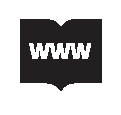
\includegraphics[height=1em]{../icons/www.eps}} Find the answers with the shortcodes:
 \par \begin{tabular}[h]{cccccc}
 (1.) ljh   \end{tabular}
\end{exercises}

    \label{m38812*cid4}
      \label{m38812*uid1}
\subsection*{Vector notation}
            \nopagebreak
Vectors are different to scalars and must have their own notation. There are many ways of writing the symbol for a vector. In this book vectors will be shown by symbols with an arrow pointing to the right above it. For example, $\stackrel{\to }{F}$, $\stackrel{\to }{W}$ and $\stackrel{\to }{v}$ represent the vectors of force, weight and velocity, meaning they have both a magnitude \textit{and} a direction.

Sometimes just the magnitude of a vector is needed. In this case, the arrow is omitted. In other words, $F$ represents the \textit{magnitude} of the force vector $\stackrel{\to }{F}$. \par 
      \label{m38812*uid2}

\section*{Graphical representation of vectors}
            \nopagebreak
        \label{m38812*id186285}Vectors are drawn as arrows. An arrow has both a magnitude (how long it is) and a direction (the direction in which it points). The starting point of a vector is known as the \textsl{tail} and the end point is known as the \textsl{head}.\par 
    \setcounter{subfigure}{0}
% \begin{minipage}{0.5\textwidth}
\begin{figure}[H]
\begin{center}
\begin{pspicture}(0,-1)(5,1)
%\psgrid[gridcolor=lightgray]
\SpecialCoor
\psline{->}(0,0)({1.5;0})\psdot(0,0)
\rput(2.5,0){\psdot(0,0)\psline{->}(0,0)({2;25})}
\rput(3,0){\psdot(0,0)\psline{->}(0,0)({2;345})}
\psline{->}(1.8,0.8)(1.8,-0.8)\psdot(1.8,0.8)
\end{pspicture}
\end{center}
\caption{Examples of vectors}
\end{figure}
% \end{minipage}
% \begin{minipage}{0.5\textwidth}
\begin{figure}[H]
\begin{center}
\begin{pspicture}(0,-0.6)(5,0.6)
%\psgrid[gridcolor=lightgray]
\psline{->}(0,0)(5,0)
\pcline[offset=8pt]{|-|}(0,0)(5,0)
\lput*{:U}{magnitude}
\psdot(0,0)
\uput[d](0,0){tail}
\uput[d](5,0){head}
\end{pspicture}
\end{center}
\caption{Parts of a vector}
\end{figure}
% \end{minipage}       
    \label{m38812*cid5}

\subsection*{Directions}
            \nopagebreak
      \label{m38812*id187219}There are many acceptable methods of writing vectors. As long as the vector has a magnitude and a direction, it is most likely acceptable. These different methods come from the different methods of representing a direction for a vector.\par 
      \label{m38812*uid5}
            \subsubsection*{Relative Directions}
            \nopagebreak
        \label{m38812*id187233}The simplest way to show direction is with relative directions: to the left, to the right, forward, backward, up and down.\par 
      \label{m38812*uid6}
            \subsubsection*{Compass Directions}
            \nopagebreak
        \label{m38812*id187246}Another common method of expressing directions is to use the points of a compass: North, South, East, and West.
If a vector does not point exactly in one of the compass directions, then we use an angle. 
For example, we can have a vector pointing $40{}^{\circ }$ North of West. Start with the vector pointing along the West direction (look at the dashed arrow below), then rotate the vector towards the north until there is a $40{}^{\circ }$ angle between the vector and the West direction (the solid arrow below).
The direction of this vector can also be described as: W $40{}^{\circ }$ N (West $40{}^{\circ }$ North); or N $50{}^{\circ }$ W (North $50{}^{\circ }$ West).\\ \\
    \setcounter{subfigure}{0}
\begin{minipage}{.5\textwidth}
\begin{center}
% \begin{pspicture}(-1.2,-1.4)(1.2,1.4)
% \pscompass
% \end{pspicture}
\includegraphics[width=.4\textwidth]{photos/ecastro.jpg}
\end{center}
\end{minipage}
\begin{minipage}{.5\textwidth}
%\begin{center}
%\begin{pspicture}(-2,-0.2)(2,0.2)
%\psgrid[gridcolor=lightgray]
%\psline{->}(1.5,0)(-1.5,0)
%\end{pspicture}
%\end{center}
\begin{center}
\begin{pspicture}(-1.5,-1)(1,1)
%\psgrid[gridcolor=lightgray]
\psarc{<-}(1,-1){1}{135}{180}
\psline{->}(1,-1)(-0.77,0.643)
\psline[linestyle=dashed]{->}(1,-1)(-1,-1)
\rput(0.35,-0.75){40$^\circ$}
\end{pspicture}
\end{center}
\end{minipage}
     \par 
      \label{m38812*uid7}
            \subsubsection*{Bearing}
            \nopagebreak
        \label{m38812*id187384}The final method of expressing direction is to use a \textsl{bearing}. A bearing is a direction relative to a fixed point.
        \label{m38812*id187393}Given just an angle, the convention is to define the angle clockwise with respect to North. So, a vector with a direction of $110{}^{\circ }$ has been rotated clockwise $110{}^{\circ }$ relative to North. A bearing is always written as a three digit number, for example $275{}^{\circ }$ or $080{}^{\circ }$ (for $80{}^{\circ }$).\par 
        \label{m38812*id187459}
    \setcounter{subfigure}{0}
\begin{center}
\begin{pspicture}(0,0)(2,2)
%\psgrid[gridcolor=lightgray]
\psline{->}(0,0)(0,2)
%\psline{->}(0,0)(1.5,-0.25)
\psline{->}(0,0)(1.88,-0.684)
\psarc{<-}(0,0){1}{-20}{90}
\rput(0.4,0.4){110$^\circ$}
\end{pspicture}
\end{center}      
        \par 
\label{m38812*secfhsst!!!underscore!!!id146}
            

\begin{exercises}{Scalars and Vectors }
            \nopagebreak
\noindent \begin{enumerate}[noitemsep, label=\textbf{\arabic*}. ] 
            \label{m38812*uid8}\item Classify the following quantities as scalars or vectors:
\label{m38812*id187490}\begin{enumerate}[noitemsep, label=\textbf{\alph*}. ] 
            \label{m38812*uid9}\item 12 km
\label{m38812*uid10}\item 1 m south
\label{m38812*uid11}\item $2\phantom{\rule{2pt}{0ex}}\text{m}\ensuremath{\cdot}{\text{s}}^{-1}$, $45{}^{\circ }$\label{m38812*uid12}\item $075{}^{\circ }$, 2 cm
\label{m38812*uid13}\item $100\phantom{\rule{2pt}{0ex}}\text{k}\ensuremath{\cdot}{\text{h}}^{-1}$, $0{}^{\circ }$\end{enumerate}
\item Use two different notations to write down the direction of the vector in each of the following diagrams:     \begin{center}
\scalebox{1} % Change this value to rescale the drawing.
{
\begin{pspicture}(0,-0.86)(11.360068,1.46)
\psline[linewidth=0.04cm,arrowsize=0.05291667cm 2.0,arrowlength=1.4,arrowinset=0.4]{->}(1.227168,-0.76)(1.247168,1.44)
\psline[linewidth=0.04cm,linestyle=dotted,dotsep=0.16cm,arrowsize=0.05291667cm 2.0,arrowlength=1.4,arrowinset=0.4]{->}(4.207168,-0.78)(6.807168,-0.8)
\psline[linewidth=0.04cm,arrowsize=0.05291667cm 2.0,arrowlength=1.4,arrowinset=0.4]{->}(4.207168,-0.78)(5.947168,1.22)
\psarc[linewidth=0.04,arrowsize=0.05291667cm 2.0,arrowlength=1.4,arrowinset=0.4]{<-}(4.697168,-0.79){0.65}{0.0}{83.659805}
\rput(4.8546534,-0.555){\small $60^{\circ}$}
\psline[linewidth=0.04cm,linestyle=dotted,dotsep=0.16cm,arrowsize=0.05291667cm 2.0,arrowlength=1.4,arrowinset=0.4]{->}(11.007168,1.42)(11.027168,-0.84)
\psline[linewidth=0.04cm,arrowsize=0.05291667cm 2.0,arrowlength=1.4,arrowinset=0.4]{->}(11.027168,1.4)(9.607168,-0.68)
\psarc[linewidth=0.04,arrowsize=0.05291667cm 2.0,arrowlength=1.4,arrowinset=0.4]{<-}(10.687168,0.88){0.52}{234.46233}{314.56595}
\rput(10.794653,0.645){\small $40^{\circ}$}
\rput(0.113310546,1.225){a.}
\rput(3.870166,1.245){b.}
\rput(9.453574,1.245){c.}
\end{pspicture} 
}
\end{center}
 \end{enumerate}

\raisebox{-0.2em}{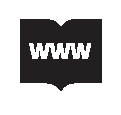
\includegraphics[height=1em]{../icons/www.eps}} Find the answers with the shortcodes:
 \par \begin{tabular}[h]{cccccc}
 (1.) l4s  &  (2.) l4H  & \end{tabular}
\end{exercises}
            \subsection*{Drawing Vectors}
            \nopagebreak
      \label{m38812*id187709}In order to draw a vector accurately we must represent its magnitude properly and
include a reference direction in the diagram. A scale allows us to
translate the length of the arrow into the vector's magnitude. For
instance if one chooses a scale of 1 cm = 2 N (1 cm represents 2 N), a
force of 20 N towards the East would be represented as an arrow 10 cm
long. The points of a compass are often used to show direction or alternatively an arrow pointing in the reference direction.  
      \label{m38812*id187716}
    \setcounter{subfigure}{0}
\begin{center}
\begin{pspicture}(0,-0.2)(10,0.6)
%\psgrid[gridcolor=lightgray]
\psline[arrowscale=2]{->}(0,0)(10,0)
\pcline[offset=8pt]{|-|}(0,0)(10,0)
\lput*{:U}{20 N}
\end{pspicture}
\scalebox{0.7}{\pscompass}
\end{center}      
      \par 
      \label{m38812*id187725}
        \textbf{Method: Drawing Vectors}
        \label{m38812*id187736}\begin{enumerate}[noitemsep, label=\textbf{\arabic*}. ] 
            \label{m38812*uid18}\item Decide upon a scale and write it down.
            \item Decide on a reference direction
\label{m38812*uid19}\item Determine the length of the arrow representing the vector, by using the scale.
\label{m38812*uid20}\item Draw the vector as an arrow. Make sure that you fill in the arrow head.
\label{m38812*uid21}\item Fill in the magnitude of the vector.
\end{enumerate}


\begin{wex}{Drawing vectors I}
{
Draw the following vector quantity: $\stackrel{\to }{v}$ =  6 \ms north
}
{
\westep{Decide on a scale and write it down.}
1 cm = 2 \ms
\westep{Decide on a reference direction}

\scalebox{1} % Change this value to rescale the drawing.
{
\begin{pspicture}(0,0)(8,1.5)
\psline{->}(1,0)(1,1)
\rput(1,1.2){N}
\rput(4,0.5){North will point up the page}
\end{pspicture} 
}
\westep{Determine the length of the arrow at the specific scale.}
If 1 cm = 2 \ms, then 6 \ms = 3 cm
\westep{Draw the vector as an arrow.}

Scale used: 1 cm = 2 \ms\\
\begin{center}
\begin{pspicture}(0,-1.3091797)(4.3466406,1.3291796)
\psline[linewidth=0.04cm,arrowsize=0.05291667cm 2.0,arrowlength=1.4,arrowinset=0.4]{->}(0.104746096,0.45082033)(0.12474609,0.9708203)
\usefont{T1}{ptm}{m}{n}
\rput(0.13456054,1.1558204){N}
\psline[linewidth=0.04cm,arrowsize=0.05291667cm 2.0,arrowlength=1.4,arrowinset=0.4]{->}(1.5047461,-1.2891797)(1.5047461,1.0908203)
\usefont{T1}{ptm}{m}{n}
\rput(2.957959,-0.26417968){6 $\mathsf{m\cdot s^{-1}}$}
\end{pspicture} 
\end{center}
%Direction = North\\
%\begin{center}
%\begin{pspicture}(-0.7,0)(0.2,3)
%\psgrid[gridcolor=lightgray]
%\psline[arrowscale=2]{->}(0,0)(0,3)
%\rput(-0.7,1.5){6 \ms}
%\pcline[offset=8pt]{|-|}(0,0)(0,3)
%\lput*{:U}{3 cm}
%\end{pspicture}
%\end{center}}
}
\end{wex}

\begin{wex}{Drawing vectors 2}
{
Draw the following vector quantity: $\stackrel{\to }{s}$ =  16 m east
}
{
\westep{Decide on a scale and write it down.}
1 cm = 4 m
\westep{Decide on a reference direction}
\scalebox{1} % Change this value to rescale the drawing.
{
\begin{pspicture}(0,0)(8,1.5)
\psline{->}(1,0)(1,1)
\rput(1,1.2){N}
\rput(4,0.5){North will point up the page}
\end{pspicture} 
}
\westep{Determine the length of the arrow at the specific scale.}
If 1 cm = 4 m, then 16 m = 4 cm
\westep{Draw the vector as an arrow}
\noindent Scale used: 1 cm = 4 m\\
Direction = East\\
\begin{center}
\begin{pspicture}(0,-0.7391797)(4.16,0.7591797)
\psline[linewidth=0.04cm,arrowsize=0.05291667cm 2.0,arrowlength=1.4,arrowinset=0.4]{->}(3.76,-0.11917969)(3.78,0.4008203)
\rput(3.7898145,0.5858203){N}
\psline[linewidth=0.04cm,arrowsize=0.05291667cm 2.0,arrowlength=1.4,arrowinset=0.4]{->}(0.0,-0.6991797)(4.14,-0.7191797)
\rput(1.828125,-0.3941797){16 m}
\end{pspicture} 
%\begin{pspicture}(0,0)(4,0.6)
%\psgrid[gridcolor=lightgray]
%\psline[arrowscale=2]{->}(0,0)(4,0)
%\rput(2,0.4){16 m}
%\pcline[offset=8pt]{|-|}(0,0)(4,0)
%\lput*{:U}{4 cm}
%\end{pspicture}
\end{center}

}
\end{wex}


\label{m38812*secfhsst!!!underscore!!!id228}
\begin{exercises}{Drawing Vectors}
            \nopagebreak
            \label{m38812*id188088}Draw each of the following vectors to scale. Indicate the scale that you have used:
      \label{m38812*id188094}\begin{enumerate}[noitemsep, label=\textbf{\arabic*}. ] 
            \label{m38812*uid30}\item 12 km south
\label{m38812*uid31}\item 1,5 m N $45{}^{\circ }$ W
\label{m38812*uid32}\item $1\phantom{\rule{2pt}{0ex}}\text{m}\ensuremath{\cdot}\text{s}{}^{-1}$, $20{}^{\circ }$ East of North
\label{m38812*uid33}\item $50\phantom{\rule{2pt}{0ex}}\text{km}\ensuremath{\cdot}\text{h}{}^{-1}$, $085{}^{\circ }$\label{m38812*uid34}\item 5 mm, $225{}^{\circ }$\end{enumerate}
                \par 
  \label{m38812**end}
\par \raisebox{-0.2em}{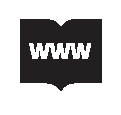
\includegraphics[height=1em]{../icons/www.eps}} Find the answers with the shortcodes:
 \par \begin{tabular}[h]{cccccc}
 (1.) l46  & \end{tabular}
\end{exercises}
         

\section{Properties of vectors}
    \nopagebreak
%            \label{m38813} $ \hspace{-5pt}\begin{array}{cccccccccccc}   \end{array} $ \hspace{2 pt}\raisebox{-0.2em}{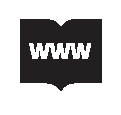
\includegraphics[height=1em]{../icons/www.eps}} {(section shortcode: P10092 )} 
    \label{m38813*cid7}
      \label{m38813*id188277}

Vectors are mathematical objects and we will now study some of their mathematical properties. 

If two vectors have the same magnitude (size) \textit{and} the same direction, then we call them equal to each other. For example, if we have two forces,  $\stackrel{\to }{F_{1}} = 20$ N \textit{in the upward direction} and $\stackrel{\to }{F_{2}} = 20$ N \textit{in the upward direction}, then we can say that $\stackrel{\to }{F_{1}} = \stackrel{\to }{F_{2}}$.

%need to understand the mathematical properties of vectors, like adding and subtracting.
%      \label{m38813*id188281}For all the examples in this section, we will use displacement as our vector quantity. 
%      \label{m38813*id188286}Displacement is defined as the distance together with direction of the straight line joining a final point to an initial point.
%      \label{m38813*id188290}Remember that displacement is just one example of a vector. We could just as well have decided to use forces or velocities to illustrate the properties of vectors.

\Definition{Equality of vectors}{Two vectors are equal if they have the \textbf{same} magnitude and the \textbf{same} direction.}

Just like scalars which can have positive or negative values, vectors can also be positive or negative. 
A negative vector is a vector which points in the direction \textit{opposite} to the \textbf{reference positive direction}. 
For example, if in a particular situation, we define the upward direction as the reference positive direction, then a force $\stackrel{\to }{F_{1}} = 30$ N \textit{downwards} would be a \textit{negative vector} and could also be written as $\stackrel{\to }{F_{1}} = -30$ N. In this case, the negative (-) sign indicates that the direction of $\stackrel{\to }{F_{1}}$ is opposite to that of the reference positive direction.

\Definition{Negative vector}{A negative vector is a vector that has the \textit{opposite} direction to the reference positive direction.}

Like scalars, vectors can also be added and subtracted. We will investigate how to do this next.

\label{m38813*uid35}
\subsection*{Addition and subtraction of vectors}
            \nopagebreak
        \label{m38813*id188304}

\subsubsection{Adding vectors}
When vectors are added, we need to take into account \textit{both} their magnitudes \textit{and} directions. 

For example, imagine the following. You and a friend are trying to move a heavy box. You stand behind it and push forwards with a force $\stackrel{\to }{F_{1}}$ and your friend stands in front and pulls it towards them with a force $\stackrel{\to }{F_{2}}$. The two forces are in the \textit{same} direction (i.e. forwards) and so the total force acting on the box is:

\begin{minipage}{0.5\textwidth}
\begin{center}
\scalebox{0.7} % Change this value to rescale the drawing.
{
\begin{pspicture}(0,-1.18)(5.62,1.18)
\psframe[linewidth=0.04,dimen=outer](3.94,1.18)(1.58,-1.18)
\psline[linewidth=0.04cm,arrowsize=0.05291667cm 2.0,arrowlength=1.4,arrowinset=0.4]{->}(0.0,-0.08)(1.64,-0.1)
\psline[linewidth=0.04cm,arrowsize=0.05291667cm 2.0,arrowlength=1.4,arrowinset=0.4]{->}(3.96,-0.12)(5.6,-0.12)
\usefont{T1}{ptm}{m}{n}
\rput(0.7814551,0.205){$\stackrel{\to }{F_{1}}$}
\usefont{T1}{ptm}{m}{n}
\rput(4.741455,0.205){$\stackrel{\to }{F_{2}}$}
\end{pspicture} 
}
\end{center}
\end{minipage}
\begin{minipage}{0.5\textwidth}
\begin{equation*}
\stackrel{\to }{F_{Tot}} = \stackrel{\to }{F_{1}} + \stackrel{\to }{F_{2}}
\end{equation*}
\end{minipage}

It is very easy to understand the concept of vector addition through an activity using the \textbf{displacement} vector.  \\
Displacement is the change in an object's position. It is a vector that points from the initial position to the final position. \\

\begin{activity}{Adding vectors}
\textbf{Materials:} masking tape \\
\textbf{Method:} \\
Tape a line of masking tape horizontally across the floor. This will be your starting point. \\
\textit{Task 1}:\\
Take 2 steps in the forward direction. Use a piece of masking tape to mark your end point and label it \textbf{A}. Then take another 3 steps in the forward direction. Use masking tape to mark your final position as \textbf{B}. Make sure you try to keep your steps all the same length! \\
\textit{Task 2}:\\
Go back to your starting line. Now take 3 steps forward. Use a piece of masking tape to mark your end point and label it \textbf{B}. Then take another 2 steps forward and use a new piece of masking tape to mark your final position as \textbf{A}. \\
\textbf{Discussion:}\\
What do you notice?\\
\begin{enumerate}[noitemsep, label=\textbf{\arabic*}.]
\item In \textit{Task 1}, the first 2 steps represent a displacement vector and the second 3 steps also form a displacement vector. If we did not stop after the first 2 steps, we would have taken 5 steps in the forward direction in total. Therefore, if we add the displacement vectors for 2 steps and 3 steps, we should get a total of 5 steps in the forward direction. 
\item It does not matter whether you take 3 steps forward and then 2 steps, or two steps followed by another 3 steps. Your final position is the same! The order of the addition does not matter!
\end{enumerate}
\end{activity}

We can represent vector addition graphically, based on the activity above. Draw the vector for the first two steps forward, followed by the vector with the next three steps forward. 
        \label{m38813*id188318}
    \setcounter{subfigure}{0}
	\begin{figure}[H] % horizontal\label{m38813*id188322}
\begin{center}
\begin{pspicture}(-6,-1)(5,0.5)%%\psgrid
%\psgrid[gridcolor=lightgray]
\uput[u](-5,0){2 steps}
\psline[linewidth=0.04cm]{->}(-6,0)(-4,0)
\rput(-3.8,0){+}
\uput[u](-2.1,0){3 steps}
\psline[linecolor=blue,linewidth=0.04cm]{->}(-3.6,0)(-0.6,0)
\rput(-0.4,0.){=}
\psline[linewidth=0.04cm]{->}(-0.2,0)(1.8,0)
\psline[linecolor=blue,linewidth=0.04cm]{->}(1.8,0)(4.8,0)
\rput(-0.4,-1){=}
\uput[u](2.3,-1){5 steps}
\psline[linewidth=0.04cm]{->}(-0.2,-1)(4.8,-1)
\end{pspicture}
\end{center}
 \end{figure} 

        \label{m38813*id188328}We add the second vector at the end of the first vector, since this is where we now are after the first vector has acted. The vector from the tail of the
first vector (the starting point) to the head of the second vector (the end
point) is then the sum of the vectors. 
%This is called the \textbf{head-to-tail} method of vector addition.\par 

\label{m38813*id188340}As you can convince yourself, the order in which you add vectors does
not matter. In the example above, if you decided to first go 3 steps
forward and then another 2 steps forward, the end result would still be 5
steps forward.

\subsubsection{Subtracting vectors}

Let's go back to the problem of the heavy box that you and your friend are trying to move. 
If you didn't communicate properly first, you both might think that you should pull in your own directions!
Imagine you stand behind the box and pull it towards you with a force $\stackrel{\to }{F_{1}}$ and your friend stands at the front of the box and pulls it towards them with a force $\stackrel{\to }{F_{2}}$. In this case the two forces are in \textit{opposite} directions. If we define the direction your friend is pulling in as \textit{positive} then the force you are exerting must be \textit{negative} since it is in the opposite direction. We can write the total force exerted on the box as the sum of the individual forces:

\begin{minipage}{0.5\textwidth}
\begin{center}
\scalebox{0.7} % Change this value to rescale the drawing.
{
\begin{pspicture}(0,-1.18)(5.62,1.18)
\psframe[linewidth=0.04,dimen=outer](3.94,1.18)(1.58,-1.18)
\psline[linewidth=0.04cm,arrowsize=0.05291667cm 2.0,arrowlength=1.4,arrowinset=0.4]{<-}(0.0,-0.1)(1.64,-0.1)
\psline[linewidth=0.04cm,arrowsize=0.05291667cm 2.0,arrowlength=1.4,arrowinset=0.4]{->}(3.96,-0.12)(5.6,-0.12)
\rput(0.7814551,0.205){$\stackrel{\to }{F_{1}}$}
\rput(4.741455,0.205){$\stackrel{\to }{F_{2}}$}
\end{pspicture} 
}
\end{center}
\end{minipage}
\begin{minipage}{0.5\textwidth}
\begin{eqnarray*}
\stackrel{\to }{F_{Tot}} & = & \stackrel{\to }{F_{2}} + (-\stackrel{\to }{F_{1}}) \\
& = & \stackrel{\to }{F_{2}} - \stackrel{\to }{F_{1}}
\end{eqnarray*}
\end{minipage}

What you have done here is actually to subtract two vectors! This is the same as adding two vectors which have opposite directions.

As we did before, we can illustrate vector subtraction nicely using displacement vectors. 
If you take 5 steps forward and then subtract 3 steps forward you are left with only two steps forward:

\begin{center}
\begin{pspicture}(-6,-0.5)(5,0.5)%%\psgrid
%\psgrid[gridcolor=lightgray]
\rput(-3.5,0.25){{5 steps}}
\psline[linewidth=0.04cm]{->}(-6,0)(-1,0)
\rput(-0.8,0){-}
\rput(1.1,0.25){{3 steps}}
\psline[linecolor=blue,linewidth=0.04cm]{->}(-0.6,0)(2.6,0)
\rput(2.8,0.){=}
\psline[linewidth=0.04cm]{->}(3.0,0)(5.0,0)
\rput(4.0,0.25){{2 steps}}
\end{pspicture}
\end{center}

What did you physically do to subtract 3 steps? You originally took 5 steps forward but then you took 3 steps \textit{backward} to land up back with only 2 steps forward. That backward displacement is represented by an arrow pointing to the left (backwards) with length 3. The net result of
adding these two vectors is 2 steps forward:

\begin{center}
\begin{pspicture}(-6,-0.5)(5,0.5)%%\psgrid
%\psgrid[gridcolor=lightgray]
\uput[u](-3.5,0){{5 steps}}
\psline[linewidth=0.04cm]{->}(-6,0)(-1,0)
\rput(-0.8,0){+}
\uput[u](1.1,0){{3 steps}}
\psline[linecolor=blue,linewidth=0.04cm]{<-}(-0.6,0)(2.6,0)
\rput(2.8,0.){=}
\psline[linewidth=0.04cm]{->}(3.0,0)(5.0,0)
\uput[u](4.0,0){{2 steps}}
\end{pspicture}
\end{center}

Thus, subtracting a vector from another is the same as adding a vector in the opposite direction (i.e. subtracting 3 steps forwards is the same
as adding 3 steps backwards). 

\Tip{Subtracting a vector from another is the same as adding a vector in the opposite direction.}


\subsubsection{Resultant and equilibrant vectors}

\label{m38813*id188345}The final quantity you get when adding or subtracting vectors is called the \textbf{resultant vector}. In other words, the individual vectors can be replaced by the
resultant -- the overall effect is the same.

\Definition{  Resultant vectors } { The resultant vector is the single vector whose effect is the same as the individual vectors acting together.    } 

We can illustrate the concept of the resultant vector by considering our two situations in using forces to move the heavy box. In the first case (on the left), you and your friend are applying forces in the same direction. The resultant force will be the sum of your two applied forces in that direction. In the second case (on the right), the forces are applied in opposite directions and the resultant force will be the difference between them. \\

\begin{minipage}[t]{0.5\textwidth}
\begin{center}
Forces are applied in the same direction \\
(positive direction to the right)\par \\

\scalebox{0.8} % Change this value to rescale the drawing.
{
%\begin{pspicture}(0,-1.06)(6.88,1.06)
\begin{pspicture}(0,-1.06)(6.88,1.5)
\psframe[linewidth=0.04,dimen=outer](4.94,1.06)(2.82,-1.06)
\psline[linewidth=0.04cm,arrowsize=0.05291667cm 2.0,arrowlength=1.4,arrowinset=0.4]{->}(0.0,0.0)(2.86,0.0)
\psline[linewidth=0.04cm,arrowsize=0.05291667cm 2.0,arrowlength=1.4,arrowinset=0.4]{->}(4.92,0.0)(6.86,0.0)
\rput(1.4814551,0.725){$\stackrel{\to }{F_{1}}$}
\rput(5.701455,0.725){$\stackrel{\to }{F_{2}}$}
\rput(1.4551758,0.265){(20 \ \mathsf{N})}
\rput(5.6151757,0.265){(15 \ \mathsf{N})}
\end{pspicture} 
}
\begin{eqnarray*}
\stackrel{\to }{F_{R}} &=& \stackrel{\to }{F_{1}} + \stackrel{\to }{F_{2}} \\
&=& 20 \ \mathsf{N} + 15 \ \mathsf{N} \\
& = & 35 \ \mathsf{N} \ \mathsf{\textit{to the right}}
\end{eqnarray*} \par \\
\end{center}
\end{minipage}
\begin{minipage}[t]{0.5\textwidth}
\begin{center}
Forces are applied in opposite directions \\
(positive direction to the right)\par \\

\scalebox{0.8} % Change this value to rescale the drawing.
{
\begin{pspicture}(0,-1.06)(6.88,1.06)
\psframe[linewidth=0.04,dimen=outer](4.94,1.06)(2.82,-1.06)
\psline[linewidth=0.04cm,arrowsize=0.05291667cm 2.0,arrowlength=1.4,arrowinset=0.4]{<-}(0.0,0.0)(2.86,0.0)
\psline[linewidth=0.04cm,arrowsize=0.05291667cm 2.0,arrowlength=1.4,arrowinset=0.4]{->}(4.92,0.0)(6.86,0.0)
\rput(1.4814551,0.725){$\stackrel{\to }{F_{1}}$}
\rput(5.701455,0.725){$\stackrel{\to }{F_{2}}$}
\rput(1.4551758,0.265){(20 \ \mathsf{N})}
\rput(5.6151757,0.265){(15 \ \mathsf{N})}
\end{pspicture} 
}
\begin{eqnarray*}
\stackrel{\to }{F_{R}} &=& \stackrel{\to }{F_{2}} + (\stackrel{\to }{-F_{2}}) \\
&=& \stackrel{\to }{F_{2}} - \stackrel{\to }{F_{1}} \\
&=& 15 \ \mathsf{N} - 20 \ \mathsf{N} \\
& = & -5 \ \mathsf{N} \\
& = & 5 \ \mathsf{N} \ \mathsf{\textit{to the left}}
\end{eqnarray*} \par \\
\end{center}
\end{minipage}

\begin{minipage}[t]{0.5\textwidth}
\begin{center}
\scalebox{0.8} % Change this value to rescale the drawing.
{
\begin{pspicture}(0,-1.06)(5.06,1.06)
\psframe[linewidth=0.04,dimen=outer](2.12,1.06)(0.0,-1.06)
\psline[linewidth=0.04cm,arrowsize=0.05291667cm 2.0,arrowlength=1.4,arrowinset=0.4]{->}(2.1,0.0)(5.04,0.0)
\rput(3.551455,0.730){$\stackrel{\to }{F_{R}}$}
\rput(3.5351758,0.225){(35 \ \mathsf{N})}
\end{pspicture} 
}
\end{center}
\end{minipage}
\begin{minipage}[t]{0.5\textwidth}
\begin{center}
\scalebox{0.8} % Change this value to rescale the drawing.
{
\begin{pspicture}(0,-1.06)(3.5010157,1.06)
\psframe[linewidth=0.04,dimen=outer](3.5010157,1.06)(1.3810157,-1.06)
\rput(0.6324707,0.730){$\stackrel{\to }{F_{R}}$}
\rput(0.8461914,0.225){(5 \ \mathsf{N})}
\psline[linewidth=0.04cm,arrowsize=0.05291667cm 2.0,arrowlength=1.4,arrowinset=0.4]{->}(1.4210156,0.0)(0.58101565,0.0)
\end{pspicture} 
}
\end{center}
\end{minipage} \\

There is a special name for the vector which has the same magnitude as the resultant vector but the \textit{opposite} direction: the \textbf{equilibrant}. If you add the resultant vector and the equilibrant vectors together, the answer is always zero because the equilibrant cancels the resultant out.

\Definition{Equilibrant}{ The equilibrant is the vector which has the \textit{same magnitude} but \textit{opposite direction} to the resultant vector.}

If you refer to the pictures of the heavy box before, the equilibrant forces for the two situations would look like: \par

\begin{minipage}[t]{0.5\textwidth}
\begin{center}
\scalebox{0.8} % Change this value to rescale the drawing.
{
\begin{pspicture}(0,-1.06)(7.74,1.06)
\psframe[linewidth=0.04,dimen=outer](4.92,1.06)(2.8,-1.06)
\rput(6.131455,0.665){$\stackrel{\to }{F_{R}}$}
\rput(6.1351757,0.245){(35 \ \mathsf{N})}
\psline[linewidth=0.04cm,linecolor=white,arrowsize=0.05291667cm 2.0,arrowlength=1.4,arrowinset=0.4]{->}(2.78,0.0)(1.94,0.0)
\psline[linewidth=0.04cm,arrowsize=0.05291667cm 2.0,arrowlength=1.4,arrowinset=0.4]{->}(4.9,-0.02)(7.72,-0.02)
\psline[linewidth=0.04cm,arrowsize=0.05291667cm 2.0,arrowlength=1.4,arrowinset=0.4]{->}(2.82,-0.02)(0.0,-0.02)
\rput(1.4614551,0.685){$\stackrel{\to }{F_{E}}$}
\rput(1.4751757,0.245){(35 \ \mathsf{N})}
\end{pspicture} 
}
\begin{eqnarray*}
\stackrel{\to }{F_{E}} &=& -\stackrel{\to }{F_{R}} \\
&=& 35 \ \mathsf{N} \ \mathsf{\textit{to the left}}
\end{eqnarray*}
\end{center}
\end{minipage}
\begin{minipage}[t]{0.5\textwidth}
\begin{center}
\scalebox{0.8} % Change this value to rescale the drawing.
{
\begin{pspicture}(0,-1.06)(4.46291,1.06)
\psframe[linewidth=0.04,dimen=outer](3.2210157,1.06)(1.1010156,-1.06)
\rput(3.7624707,0.725){$\stackrel{\to }{F_{E}}$}
\rput(3.7461915,0.245){(5N)}
\psline[linewidth=0.04cm,linecolor=white,arrowsize=0.05291667cm 2.0,arrowlength=1.4,arrowinset=0.4]{->}(1.0810156,0.0)(0.24101563,0.0)
\psline[linewidth=0.04cm,arrowsize=0.05291667cm 2.0,arrowlength=1.4,arrowinset=0.4]{->}(1.1210157,-0.02)(0.021015625,-0.02)
\rput(0.6324707,0.725){$\stackrel{\to }{F_{R}}$}
\rput(0.6261914,0.205){(5N)}
\psline[linewidth=0.04cm,arrowsize=0.05291667cm 2.0,arrowlength=1.4,arrowinset=0.4]{->}(3.2010157,-0.02)(4.301016,-0.02)
\end{pspicture} 
}
\begin{eqnarray*}
\stackrel{\to }{F_{E}} &=& -\stackrel{\to }{F_{R}} \\
&=& 5 \ \mathsf{N} \ \mathsf{\textit{to the right}}
\end{eqnarray*}
\end{center}
\end{minipage} 


\section{Techniques of vector addition}

Now that you have learned about the mathematical properties of
vectors, we return to vector addition in more detail. There are a number of
techniques of vector addition. These techniques fall into two main categories - graphical and algebraic techniques.

\subsection*{Graphical techniques}
Graphical techniques involve drawing accurate scale diagrams to denote
individual vectors and their resultants. We will look at just one graphical method: the head-to-tail method.

\subsubsection*{The head-to-tail method}
In describing the mathematical properties of vectors we used
displacements and the head-to-tail graphical method of vector addition
as an illustration. The head-to-tail method of graphically adding vectors is a standard method that must be understood.\\

\textbf{Method: Head-to-Tail Method of Vector Addition}
\begin{enumerate}[noitemsep, label=\textbf{\arabic*}.]
\item{Draw a rough sketch of the situation.}
\item{Choose a scale and include a reference direction.}
\item{Choose any of the vectors and draw it as an arrow in the
correct direction and of the correct length -- remember to put an
arrowhead on the end to denote its direction.}
\item{Take the next vector and draw it as an arrow starting from the
arrowhead of the first vector in the correct direction and of the
correct length.}
\item{Continue until you have drawn each vector -- each time starting
from the head of the previous vector. In this way, the vectors to be
added are drawn one after the other head-to-tail.}
\item{The resultant is then the vector drawn from the tail of the
first vector to the head of the last. Its magnitude can be
determined from the length of its arrow using the scale. Its
direction too can be determined from the scale diagram.}
\end{enumerate} \par


\label{m38813*id188482}Let's consider some more examples of vector addition using displacements. The arrows tell you how far to move and in what direction. Arrows to the right correspond to steps forward, while arrows to the left correspond to steps backward. Look at all of the examples below and check them.\par 
        \label{m38813*id186651}
    \setcounter{subfigure}{0}
	\begin{figure}[H] % horizontal\label{m38813*id186654}
\begin{center}
\begin{pspicture}(0,0)(8,0.5)%%\psgrid
%\psgrid[gridcolor=lightgray]
\uput[u](0.48,0){1 step}
\psline[linewidth=0.04cm]{->}(1,0)
\rput(1.3,0){+}
\rput[u](2.08,0.325){1 step}
\psline[linecolor=blue,linewidth=0.04cm]{->}(1.6,0)(2.6,0)
\rput(2.9,-0.025){=}
\uput[u](4.18,0){2 steps}
\psline[linewidth=0.04cm]{->}(3.2,0)(4.2,0)
\psline[linecolor=blue,linewidth=0.04cm]{->}(4.2,0)(5.2,0)
\rput(5.5,-0.025){=}
\uput[u](6.78,0){2 steps}
\psline[linewidth=0.04cm]{->}(5.8,0)(7.8,0)
\end{pspicture}
\end{center}
\end{figure}       
       
\label{m38813*id186661}This example says 1 step forward and then another step forward is the same as an arrow twice as long -- two steps forward.\par 
        \label{m38813*id186668}
    \setcounter{subfigure}{0}
\begin{figure}[H]
\begin{center}
 \begin{pspicture}(0,0)(8,1)%%\psgrid
%\psgrid[gridcolor=lightgray]
\rput(0.48,0.25){{1 step}}
\psline[linewidth=0.04cm]{<-}(1,0)
\rput(1.3,0){+}
\rput(2.08,0.25){{1 step}}
\psline[linecolor=blue,linewidth=0.04cm]{<-}(1.6,0)(2.6,0)
\rput(2.9,-0.025){=}
\rput(4.18,0.25){{2 steps}}
\psline[linewidth=0.04cm]{<-}(3.2,0)(4.2,0)
\psline[linecolor=blue,linewidth=0.04cm]{<-}(4.2,0)(5.2,0)
\rput(5.5,-0.025){=}
\rput(6.78,0.25){{2 steps}}
\psline[linewidth=0.04cm]{<-}(5.8,0)(7.8,0)
\end{pspicture}
\end{center}
 \end{figure}      
        \par 
        \label{m38813*id186678}This example says 1 step backward and then another step backward is the same as an arrow twice as long -- two steps backward.\par 

It is sometimes possible that you end up back where you started. In this case the net result of what you have done is that you have gone nowhere
(your start and end points are at the same place). In this case, your resultant displacement is a vector with length zero units. We use the symbol $\vec{0}$ to denote such a vector:

\begin{center}
\begin{pspicture}(-0.5,-0.5)(8,0.5)%%\psgrid
%\psgrid[gridcolor=lightgray]
\rput(0.48,0.25){{1 step}}
\psline[linewidth=0.04cm]{->}(1,0)
\rput(1.3,0){+}
\rput(2.08,0.25){{1 step}}
\psline[linecolor=blue,linewidth=0.04cm]{<-}(1.6,0)(2.6,0)
\rput(2.9,-0.025){=}
\rput(4.18,0.25){{1 step}}
%\psline[linewidth=0.04cm]{->}(3.7,0.05)(4.7,0.05)
%\psline[linecolor=blue,linewidth=0.04cm]{<-}(3.7,-0.05)(4.7,-0.05)
\psline[linewidth=0.04cm]{->}(3.7,0.0)(4.7,0.0)
\psline[linecolor=blue,linewidth=0.04cm]{<-}(3.7,-0.0)(4.7,-0.0)
\rput(4.18,-0.28){{1 step}}
\rput(5.5,0){= $\vec{0}$}
\end{pspicture}
\end{center}

\begin{center}
\begin{pspicture}(-0.5,-0.5)(8,0.5)%%\psgrid
%\psgrid[gridcolor=lightgray]
\rput(0.48,0.25){{1 step}}
\psline[linewidth=0.04cm]{<-}(1,0)
\rput(1.3,0){+}
\rput(2.08,0.25){{1 step}}
\psline[linecolor=blue,linewidth=0.04cm]{->}(1.6,0)(2.6,0)
\rput(2.9,-0.025){=}
\rput(4.18,0.25){{1 step}}
%\psline[linewidth=0.04cm]{<-}(3.7,0.05)(4.7,0.05)
%\psline[linecolor=blue,linewidth=0.04cm]{->}(3.7,-0.05)(4.7,-0.05)
\psline[linewidth=0.04cm]{<-}(3.7,0.0)(4.7,0.0)
\psline[linecolor=blue,linewidth=0.04cm]{->}(3.7,-0.0)(4.7,-0.0)
\rput(4.18,-0.28){{1 step}}
\rput(5.5,0){= $\vec{0}$}
\end{pspicture}
\end{center}     

\label{m38813*id188632}Check the following examples in the same way. Arrows up the page can be
seen as steps left and arrows down the page as steps right.\par 
\label{m38813*id188636}Try a couple to convince yourself!\par \nopagebreak

\begin{minipage}[t]{0.5\textwidth}
\begin{center}
%\begin{tabular}{cc}
\begin{pspicture}(-0.5,-1.)(2.3,1)%%\psgrid
%\psgrid[gridcolor=lightgray]
\psline[linewidth=0.04cm]{->}(0, -0.35)(0,0.35)
\rput(0.3,0.0){+}
\psline[linecolor=blue,linewidth=0.04cm]{->}(0.6,-0.35)(0.6,0.35)
\rput(0.9,0){=}
\psline[linewidth=0.04cm]{->}(1.2,-0.7)(1.2,0)
\psline[linecolor=blue,linewidth=0.04cm]{->}(1.2,0)(1.2,0.7)
\rput(1.5,0){=}
\psline[linewidth=0.04cm]{->}(1.8,-0.7)(1.8,0.7)
\end{pspicture}
%&
\end{center}
\end{minipage}
\begin{minipage}[t]{0.5\textwidth}
\begin{center}
\begin{pspicture}(-0.5,-1.)(2.3,1)%%\psgrid
%\psgrid[gridcolor=lightgray]
\psline[linewidth=0.04cm]{<-}(0, -0.35)(0,0.35)
\rput(0.3,0.0){+}
\psline[linecolor=blue,linewidth=0.04cm]{<-}(0.6,-0.35)(0.6,0.35)
\rput(0.9,0){=}
\psline[linewidth=0.04cm]{<-}(1.2,-0.7)(1.2,0)
\psline[linecolor=blue,linewidth=0.04cm]{<-}(1.2,0)(1.2,0.7)
\rput(1.5,0){=}
\psline[linewidth=0.04cm]{<-}(1.8,-0.7)(1.8,0.7)
\end{pspicture}
%\end{tabular}
\end{center}
\end{minipage}\par

\begin{minipage}[t]{0.5\textwidth}
\begin{center}
%\begin{tabular}{cc}
\begin{pspicture}(-0.5,-1.)(2.3,1)%%\psgrid
%\psgrid[gridcolor=lightgray]
\psline[linewidth=0.04cm]{<-}(0, -0.35)(0,0.35)
\rput(0.3,0.0){+}
\psline[linecolor=blue,linewidth=0.04cm]{->}(0.6,-0.35)(0.6,0.35)
\rput(0.9,0){=}
%\psline[linewidth=0.04cm]{<-}(1.2,-0.35)(1.2,0.35)
%\psline[linecolor=blue,linewidth=0.04cm]{->}(1.3,-0.35)(1.3,0.35)
\psline[linewidth=0.04cm]{<-}(1.1,-0.35)(1.1,0.35)
\psline[linecolor=blue,linewidth=0.04cm]{->}(1.1,-0.35)(1.1,0.35)
\rput(1.6,0){=}
\rput(2.0,0){$\vec{0}$}
\end{pspicture}
\end{center}
\end{minipage}
\begin{minipage}[t]{0.5\textwidth}
\begin{center}
\begin{pspicture}(-0.5,-1.)(2.3,1)%%\psgrid
%\psgrid[gridcolor=lightgray]
\psline[linewidth=0.04cm]{->}(0, -0.35)(0,0.35)
\rput(0.3,0.0){+}
\psline[linecolor=blue,linewidth=0.04cm]{<-}(0.6,-0.35)(0.6,0.35)
\rput(0.9,0){=}
%\psline[linewidth=0.04cm]{->}(1.2,-0.35)(1.2,0.35)
%\psline[linecolor=blue,linewidth=0.04cm]{<-}(1.3,-0.35)(1.3,0.35)
\psline[linewidth=0.04cm]{->}(1.1,-0.35)(1.1,0.35)
\psline[linecolor=blue,linewidth=0.04cm]{<-}(1.1,-0.35)(1.1,0.35)
\rput(1.6,0){=}
\rput(2.0,0){$\vec{0}$}
\end{pspicture}
%\end{tabular}
\end{center}
\end{minipage}
    \par
It is important to realise that the directions are not special-- `forward
and backwards' or `left and right' are treated in the same way. The same is
true of any set of parallel directions: 

\begin{minipage}[t]{0.5\textwidth}
\begin{center}
\begin{pspicture}(-0.1,-1.)(5.,1)%%\psgrid
%\psgrid[gridcolor=lightgray]
\psline[linewidth=0.04cm]{->}(0, -.35)(.7,0.35)
\rput(0.8,0.0){+}
\psline[linecolor=blue,linewidth=0.04cm]{->}(0.9,-.35)(1.6,0.35)
\rput(1.7,0){=}
\psline[linewidth=0.04cm]{->}(1.8,-0.7)(2.5,0)
\psline[linecolor=blue,linewidth=0.04cm]{->}(2.5,0)(3.2,0.7)
\rput(3.3,0){=}
\psline[linewidth=0.04cm]{->}(3.4,-0.7)(4.8,0.7)
\end{pspicture}
\end{center}
\end{minipage}
\begin{minipage}[t]{0.5\textwidth}
\begin{center}
\begin{pspicture}(-0.1,-1.)(5.,1)%%\psgrid
%\psgrid[gridcolor=lightgray]
\psline[linewidth=0.04cm]{<-}(0, -.35)(.7,0.35)
\rput(0.8,0.0){+}
\psline[linecolor=blue,linewidth=0.04cm]{<-}(0.9,-.35)(1.6,0.35)
\rput(1.7,0){=}
\psline[linewidth=0.04cm]{<-}(1.8,-0.7)(2.5,0)
\psline[linecolor=blue,linewidth=0.04cm]{<-}(2.5,0)(3.2,0.7)
\rput(3.3,0){=}
\psline[linewidth=0.04cm]{<-}(3.4,-0.7)(4.8,0.7)
\end{pspicture}
\end{center}
\end{minipage} \par


\begin{minipage}[t]{0.5\textwidth}
\begin{center}
\begin{pspicture}(-0.1,-1.)(3.5,1)%%\psgrid
%\psgrid[gridcolor=lightgray]
\psline[linewidth=0.04cm]{->}(0, -.35)(.7,0.35)
\rput(0.8,0.0){+}
\psline[linecolor=blue,linewidth=0.04cm]{<-}(0.9,-.35)(1.6,0.35)
\rput(1.7,0){=}
\psline[linewidth=0.04cm]{->}(1.8,-0.35)(2.5,.35)
%\psline[linecolor=blue,linewidth=0.04cm]{<-}(1.9,-0.35)(2.6,0.35)
\psline[linecolor=blue,linewidth=0.04cm]{<-}(1.8,-0.35)(2.5,0.35)
\rput(2.7,0){=}
\rput(3.1,0){$\vec{0}$}
\end{pspicture}
\end{center}
\end{minipage}
\begin{minipage}[t]{0.5\textwidth}
\begin{center}
\begin{pspicture}(-0.1,-1.)(3.5,1)%%\psgrid
%\psgrid[gridcolor=lightgray]
\psline[linewidth=0.04cm]{<-}(0, -.35)(.7,0.35)
\rput(0.8,0.0){+}
\psline[linecolor=blue,linewidth=0.04cm]{->}(0.9,-.35)(1.6,0.35)
\rput(1.7,0){=}
\psline[linewidth=0.04cm]{<-}(1.8,-0.35)(2.5,.35)
%\psline[linecolor=blue,linewidth=0.04cm]{->}(1.9,-0.35)(2.6,0.35)
\psline[linecolor=blue,linewidth=0.04cm]{->}(1.8,-0.35)(2.5,0.35)
\rput(2.7,0){=}
\rput(3.1,0){$\vec{0}$}
\end{pspicture}
\end{center}
\end{minipage} \par

In the above examples the separate displacements were parallel to one
another. However the same head-to-tail technique of vector addition
can be applied to vectors in any direction.

%\begin{center}
%\begin{tabular}{ccc}
%\begin{pspicture}(-0.5,-0.5)(4.0,0.5)%%\psgrid
%\psgrid[gridcolor=lightgray]
%\psline[linewidth=0.04cm]{->}(0.7,0)
%\rput(1,0){+}
%\psline[linecolor=blue,linewidth=0.04cm]{->}(1.3,-0.35)(1.3,0.35)
%\rput(1.5,-0.025){=}
%\psline[linewidth=0.04cm]{->}(1.8,-0.35)(2.5,-0.35)
%\psline[linecolor=blue,linewidth=0.04cm]{->}(2.5,-0.35)(2.5,0.35)
%\psline[linestyle=dotted]{->}(1.8,-0.35)(2.5,0.35)
%\rput(2.8,0.025){=}
%\psline[linewidth=0.04cm]{->}(3.1,-0.35)(3.8,0.35)
%\end{pspicture}
%&
%\begin{pspicture}(-0.5,-0.5)(4.0,0.5)%%\psgrid
%\psgrid[gridcolor=lightgray]
%\psline[linewidth=0.04cm]{->}(0.7,0)
%\rput(1,0){+}
%\psline[linecolor=blue,linewidth=0.04cm]{<-}(1.3,-0.35)(1.3,0.35)
%\rput(1.5,-0.025){=}
%\psline[linewidth=0.04cm]{->}(1.8,0.35)(2.5,0.35)
%\psline[linecolor=blue,linewidth=0.04cm]{<-}(2.5,-0.35)(2.5,0.35)
%\psline[linestyle=dotted]{->}(1.8,0.35)(2.5,-0.35)
%\rput(2.8,0.025){=}
%\psline[linewidth=0.04cm]{->}(3.1,0.35)(3.8,-0.35)
%\end{pspicture}
%&
%\begin{pspicture}(-0.5,-0.5)(4.0,0.5)%%\psgrid
%\psgrid[gridcolor=lightgray]
%\psline[linewidth=0.04cm]{->}(0.,-0.1)(0.7,0.1)
%\rput(1,0){+}
%\psline[linecolor=blue,linewidth=0.04cm]{->}(1.3,-0.35)(1.5,0.35)
%\rput(1.6,-0.025){=}
%\psline[linewidth=0.04cm]{->}(1.7,-0.45)(2.4,-0.25)
%\psline[linecolor=blue,linewidth=0.04cm]{->}(2.4,-0.25)(2.6,0.45)
%\psline[linestyle=dotted]{->}(1.7,-0.45)(2.6,0.45)
%\rput(2.9,0.025){=}
%\psline[linewidth=0.04cm]{->}(3.2,-0.45 )(4.1,0.45)
%\end{pspicture}
%\end{tabular}
%\end{center}




%\subsection*{Scalar Multiplication}
%What happens when you multiply a vector by a scalar (an ordinary
%number)?
%Going back to normal multiplication we know that $2 \times 2$ is just
%$2$ groups of $2$ added together to give $4$. We can adopt a similar  approach to understand how vector multiplication works.

%\begin{center}
%\begin{pspicture}(-0.5,-0.5)(6.2,0.5)%%\psgrid
%\psgrid[gridcolor=lightgray]
%\rput(0.7,0){2}
%\rput(1,0){x}
%\psline[linewidth=0.04cm]{->}(1.3,0)(2,0)
%\rput(2.3,-0.025){=}
%\psline[linewidth=0.04cm]{->}(2.6,0)(3.3,0)
%\rput(3.45,0){+}
%\psline[linewidth=0.04cm]{->}(3.6,0)(4.3,0)
%\rput(4.6,-0.025){=}
%\psline[linewidth=0.04cm]{->}(4.9,0)(6.3,0)
%\end{pspicture}
%\end{center}


\begin{wex}{Head-to-Tail Addition I}{A ship leaves harbour H and sails 6 km north to port A. From here the ship travels 12 km east to port B, before sailing 5,5 km south-west to port C. Determine the ship's resultant displacement using the head-to-tail technique of vector addition.}{

\westep{Draw a rough sketch of the situation}
It's easy to understand the problem if we first draw a quick sketch. The rough sketch should include all of the information given in the problem. All of the magnitudes of the displacements are shown. In a rough sketch one is interested in the approximate shape of the vector diagram.

\begin{center}
\begin{pspicture}(-4,-4)(4,0.5)
%\psgrid[gridcolor=lightgray]
\psline[arrowscale=2]{->}(-3.8,-3.8)(-3.8,0)
\psline[arrowscale=2,linecolor=blue]{->}(-3.8,0)(3.8,0)
\psline[arrowscale=2,linecolor=red]{->}(3.8,0)(1.11,-2.69)
\rput(-4,-3.8){H}
\rput(-4.2,-1.9){6 km}
\rput(-4,0){A}
\rput(0,0.3){12 km}
\rput(4,0){B}
\rput(3.1,-1.4){5,5 km}
\rput(1.35,-2.69){C}
\psarc{-}(3.8,0){1.4}{180}{225}
\rput(3.05,-0.35){45$^\circ$}
\psline[arrowscale=2]{->}(-3.8,-3.8)(1.11,-2.69)
\end{pspicture}
% \scalebox{0.7}{\pscompass}
\end{center}

\westep{Choose a scale and include a reference direction.}
The choice of scale depends on the actual question -- you should choose a
scale such that your vector diagram fits the page. 

It is clear from the rough sketch that choosing a scale where 1~cm represents 2~km (scale: 1~cm = 2~km) would be a good choice in this 
problem. We now start the accurate construction.

\westep{Choose any of the vectors to be summed and draw it as an arrow in the correct direction and of the correct length -- remember to put an
arrowhead on the end to denote its direction.}
Starting at the harbour H we draw the first vector 3~cm long in the direction north.

%\MarginTip{Scale: 1~cm = 2~km}
\begin{center}
\begin{pspicture}(0,0)(8,3.5)
%\psgrid[gridcolor=lightgray]
\psline[arrowscale=2]{->}(0.5,0)(0.5,3)
\uput[l](0.5,0){H}
\uput[l](0.5,1.5){6 km}
\uput[l](0.5,3){A}
\end{pspicture}
\end{center}

\westep{Take the next vector and draw it as an arrow starting from the
head of the first vector in the correct direction and of the
correct length.}
Since the ship is now at port A we draw the second vector 6~cm long starting from point A in the direction east.

\begin{center}
\begin{pspicture}(0,0)(8,3.5)
%\psgrid[gridcolor=lightgray]
\psline[arrowscale=2]{->}(0.5,0)(0.5,3)
\uput[l](0.5,0){H}
\uput[l](0.5,1.5){6 km}
\uput[l](0.5,3){A}
\psline[arrowscale=2,linecolor=blue]{->}(0.5,3)(6.5,3)
\uput[u](3.5,3){12 km}
\uput[u](6.5,3){B}
\end{pspicture}
% \scalebox{0.7}{\pscompass}
\end{center}

\westep{Take the next vector and draw it as an arrow starting from the
head of the second vector in the correct direction and of the
correct length.}
Since the ship is now at port B we draw the third vector 2,25~cm long starting from this point in the direction south-west. A protractor is required to measure the angle of 45$^\circ$.

\begin{center}
\begin{pspicture}(0,0)(8,3.5)
%\psgrid[gridcolor=lightgray]
\SpecialCoor
\psline[arrowscale=2]{->}(0.5,0)(0.5,3)
\uput[l](0.5,0){H}
\uput[l](0.5,1.5){6 km}
\uput[l](0.5,3){A}
\psline[arrowscale=2,linecolor=blue]{->}(0.5,3)(6.5,3)
\uput[u](3.5,3){12 km}
\uput[u](6.5,3){B}
\rput(6.5,3){\psline[arrowscale=2,linecolor=red]{->}(0,0)({2.25;225})
\uput[u]({2.25;225}){C}}
\uput[r](5.8,2){5,5 km}
\psarc{->}(6.5,3){1.4}{180}{225}
\rput(5.7,2.65){45$^\circ$}
\end{pspicture}
% \scalebox{0.7}{\pscompass}
\end{center}

\westep{The resultant is then the vector drawn from the tail of the
first vector to the head of the last. Its magnitude can be
determined from the length of its arrow using the scale. Its
direction too can be determined from the scale diagram.}

As a final step we draw the resultant displacement from
the starting point (the harbour H) to the end point (port C). We use a
ruler to measure the length of this arrow and a protractor to determine its direction.

\begin{center}
\begin{pspicture}(0,0)(8,3.5)
%\psgrid[gridcolor=lightgray]
\SpecialCoor
\psline[arrowscale=2]{->}(0.5,0)(0.5,3)
\uput[l](0.5,0){H}
\uput[l](0.5,1.5){3 cm = 6 km}
\uput[l](0.5,3){A}
\psline[arrowscale=2,linecolor=blue]{->}(0.5,3)(6.5,3)
\uput[u](3.5,3){6 cm = 12 km}
\uput[u](6.5,3){B}
\rput(6.5,3){\psline[arrowscale=2,linecolor=red]{->}(0,0)({2.25;225})
\uput[u]({2.25;225}){C}}
\uput[r](5.8,2){2,25 cm = 5,5 km}
\psline[linewidth=2pt]{->}(0.5,0)(4.91,1.41)
\pcline[offset=8pt,linestyle=none](0.5,0)(4.91,1.41)
\lput*{:U}{4,6 cm = 9,2 km}
\psarc{->}(0.5,0){0.9}{17.7}{90}
\rput(0.85,0.45){?}
\end{pspicture}
% \scalebox{0.7}{\pscompass}
\end{center}

\westep{Apply the scale conversion}
We now use the scale to convert the length of the resultant in the scale diagram to the actual displacement in the problem. Since we have chosen a scale of 1~cm = 2~km in this problem the resultant has a magnitude of 9,2~km. The direction can be specified in terms of the angle measured either as 072,3$^\circ$ east of north or on a bearing of 072,3$^\circ$.

\westep{Quote the final answer}
The resultant displacement of the ship is 9,2 km on a bearing of 072,3$^\circ$.}
\end{wex}
\pagebreak
\begin{wex}{Head-to-Tail Graphical Addition II}{A man walks 40 m East, then 30 m North.
\begin{enumerate}[noitemsep, label=\textbf{\arabic*}.]
\item{What was the total distance he walked?}
\item{What is his resultant displacement?}
\end{enumerate}}
{
\westep{Draw a rough sketch}
\begin{center}
\begin{pspicture}(-0.5,-0.5)(6,3)
%\psgrid[gridcolor=lightgray]
\psline[arrowscale=2]{->}(0,0)(4,0)
\psline[arrowscale=2,linecolor=blue]{->}(4,0)(4,3)
\psline[linewidth=2pt]{->}(0,0)(4,3)
\pcline[offset=8pt,linestyle=none]{-}(0,0)(4,3)
\lput*{:U}{resultant}
\uput[d](2,0){40 m}
\uput[r](4,1.5){30 m}
\end{pspicture}
% \scalebox{0.7}{\pscompass}
\end{center}

\westep{Determine the distance that the man traveled}
In the first part of his journey he traveled 40 m and in the second part he traveled 30 m. This gives us a total distance traveled of 40 m + 30 m = 70 m.

\westep{Determine his resultant displacement}
The man's resultant displacement is the {\bf vector} from where he started to where he ended. It is the vector sum of his two separate displacements. We will use the head-to-tail method of accurate construction to find this vector. 

\westep{Choose a suitable scale}
A scale of 1 cm represents 10 m (1~cm = 10~m) is a good choice here. Now we can begin the process of construction.

\westep{Draw the first vector to scale}
We draw the first displacement as an arrow 4~cm long in an eastwards direction.

\begin{center}
\begin{pspicture}(-0.5,-0.5)(6,0.5)
%\psgrid[gridcolor=lightgray]
\psline[arrowscale=2]{->}(0,0)(4,0)
\uput[d](2,0){4 cm = 40 m}
\end{pspicture}
% \scalebox{0.7}{\pscompass}
\end{center}

\westep{Draw the second vector to scale}
Starting from the head of the first vector we draw the second vector as an arrow 3~cm long in a northerly direction.

\begin{center}
\begin{pspicture}(-0.5,-0.5)(6,3)
%\psgrid[gridcolor=lightgray]
\psline[arrowscale=2]{->}(0,0)(4,0)
\psline[arrowscale=2,linecolor=blue]{->}(4,0)(4,3)
\uput[d](2,0){4 cm = 40 m}
\uput[r](4,1.5){3 cm = 30 m}
\end{pspicture}
% \scalebox{0.7}{\pscompass}
\end{center}

\westep{Determine the resultant vector}
Now we connect the starting point to the end point and
measure the length and direction of this arrow (the resultant).

\begin{center}
\begin{pspicture}(-0.5,-0.5)(6,3)
%\psgrid[gridcolor=lightgray]
\psline[arrowscale=2]{->}(0,0)(4,0)
\psline[arrowscale=2,linecolor=blue]{->}(4,0)(4,3)
\psline[linewidth=2pt]{->}(0,0)(4,3)
\pcline[offset=8pt,linestyle=none]{-}(0,0)(4,3)
\lput*{:U}{5 cm = 50 m}
\uput[d](2,0){4 cm = 40 m}
\uput[r](4,1.5){3 cm = 30 m}
\psarc{->}(0,0){1.25}{0}{36.9}
\rput(0.85,0.25){?}
\end{pspicture}
% \scalebox{0.7}{\pscompass}
\end{center}

\westep{Find the direction}
To find the direction you measure the angle between the resultant and the 40~m vector. You should get about 37$^\circ$.

\westep{Apply the scale conversion}
Finally we use the scale to convert the length of the resultant in
the scale diagram to the actual magnitude of the resultant
displacement. According to the chosen scale 1 cm = 10 m. Therefore 5 cm  represents 50 m. The resultant displacement is then 50 m 37$^\circ$ north of east.
}
\end{wex}

\subsection*{Algebraic Addition and Subtraction of Vectors}
\subsubsection*{Vectors in a Straight Line}

Whenever you are faced with adding vectors acting in a straight line (i.e. some directed left and some right, or some acting up and others down) you can use a very simple algebraic technique:\\

\begin{minipage}{\textwidth}
\textbf{Method: Addition/Subtraction of Vectors in a Straight Line}
\begin{enumerate}[noitemsep, label=\textbf{\arabic*}.]
\item{Choose a positive direction. As an example, for
situations involving displacements in the directions west and east, you
might choose west as your positive direction. In that case,
displacements east are negative.}
\item{Next simply add (or subtract) the
magnitude of the vectors using the appropriate signs.}
\item{As a final step the direction of the resultant should be included in
words (positive answers are in the positive direction, while negative
resultants are in the negative direction).}\\
\end{enumerate}
\end{minipage}

Let us consider a few examples. 

\begin{wex}{Adding vectors algebraically I}{A tennis ball is rolled towards a wall which is 10~m away from the ball. If after striking the wall the ball rolls a further 2,5~m along the ground away from the wall, calculate algebraically the ball's resultant displacement.}{
\westep{Draw a rough sketch of the situation}
\begin{center}
\begin{pspicture}(-0.5,-0.5)(6,2)
%\psgrid[gridcolor=lightgray]
\psline[linewidth=0.04cm]{->}(0,1.5)(5,1.5)
\rput(2.5,1.7){10 m}
\psline[linewidth=0.04cm]{->}(5,1)(3.75,1)
\rput(4.5,1.2){2,5 m}
\psline{-}(5,0)(5,2)
\rput(5.5,1){Wall}
\psline[linestyle=dashed]{-}(0,0)(0,2)
\rput(0,-0.2){Start}
\end{pspicture}
\end{center} 
\westep{Decide which method to use to calculate the resultant}
We know that the resultant displacement of the ball
($\vec{x}_{R}$) is equal to the sum of the ball's separate
displacements ($\vec{x}_1$ and $\vec{x}_2$):
\begin{eqnarray*}
\vec{x}_{R} & = & \vec{x}_{1} + \vec{x}_{2}
\end{eqnarray*}
Since the motion of the ball is in a straight line (i.e. the ball
moves towards and away from the wall), we can use the method of algebraic addition
just explained.
\westep{Choose a positive direction}
Let's choose the \textbf{positive} direction to be towards the wall. This means that the \textbf{negative} direction is away from the wall.
\westep{Now define our vectors algebraically}
With right positive: 
\begin{eqnarray*}
\vec{x}_{1} & = & +10,0\emm \\
\vec{x}_{2} & = & -2,5\emm 
\end{eqnarray*}

\westep{Add the vectors}
Next we simply add the two displacements to give the resultant:
\begin{eqnarray*}
\vec{x}_{R} & = & (+10\emm) + (-2,5\emm) \\
& = & (+7,5)\emm
\end{eqnarray*}
\westep{Quote the resultant}
Finally, in this case \underline{towards the wall is the positive direction}, so:
$\vec{x}_{R}$  =  7,5 m towards the wall.}
\end{wex}

\begin{wex}{Subtracting vectors algebraically I}{Suppose that a tennis ball is thrown horizontally towards a wall at an initial velocity of 3 \ms to the right. After striking the wall, the ball returns to the thrower at 2 \ms. Determine the change in velocity of the ball.}{
\westep{Draw a sketch}
A quick sketch will help us understand the problem.
\begin{center}
\begin{pspicture}(-0.5,-0.5)(4,2)
%\psgrid[gridcolor=lightgray]
\psline[linewidth=0.04cm]{->}(0,1.5)(3,1.5)
\rput(1.5,1.7){3 \ms}
\psline[linewidth=0.04cm]{->}(3,1)(1,1)
\rput(2,1.2){2 \ms}
\psline{-}(3,0)(3,2)
\rput(3.5,1){Wall}
\psline[linestyle=dashed]{-}(0,0)(0,2)
\rput(0,-0.2){Start}
\end{pspicture}
\end{center} 
\westep{Decide which method to use to calculate the resultant}
Remember that velocity is a vector. The change in the velocity of the
ball is equal to the difference between the ball's initial and final
velocities: 
\begin{equation*}
\Delta\vec{v}  =  \vec{v}_{f} - \vec{v}_{i} 
\end{equation*}

Since the ball moves along a straight line (i.e. left and right), we
can use the algebraic technique of vector subtraction just discussed.

\westep{Choose a positive direction} 
Choose the \textbf{positive} direction to be towards the wall. This means that the \textbf{negative} direction is away from the wall. 

\westep{Now define our vectors algebraically}
\begin{eqnarray*}
\vec{v}_{i} & = & +3\ems \\
\vec{v}_{f} & = & -2\ems 
\end{eqnarray*}

\westep{Subtract the vectors}
Thus, the change in velocity of the ball is:

\begin{eqnarray*}
\Delta\vec{v} & = & (-2\ems) - (+3\ems) \\
& = & (-5)\ems
\end{eqnarray*}
\westep{Quote the resultant}
Remember that in this case \underline{towards the wall means a positive velocity}, so \underline{away from the wall means a negative velocity}:
$\Delta\vec{v} =  5\ems$ away from the wall.}
\end{wex}

\begin{wex}{Adding vectors algebraically II}{A man applies a force of $5 ~\text{N}$ on a crate. The crate pushes back on the man with a force of $2~ \text{N}$. Calculate algebraically the resultant force that the man applies to the crate.}{
\westep{Draw a sketch}
A quick sketch will help us understand the problem.
\begin{center}
\begin{pspicture}(-0.5,-0.5)(4,2)
%\psgrid[gridcolor=lightgray]
\psline[linewidth=0.04cm]{->}(0,1.5)(3,1.5)
\rput(1.5,1.7){$5~\text{N}$}
\psline[linewidth=0.04cm]{->}(3,1)(1,1)
\rput(2,1.2){$2~\text{N}$}
% \psline{-}(3,0)(3,2)
% \rput(3.5,1){Wall}
% \psline[linestyle=dashed]{-}(0,0)(0,2)
% \rput(0,-0.2){Start}
\end{pspicture}
\end{center} 
\westep{Decide which method to use to calculate the resultant}
Remember that force is a vector. Since the crate moves along a straight line (i.e. left and right), we
can use the algebraic technique of vector addition just discussed.

\westep{Choose a positive direction} 
Choose the \textbf{positive} direction to be towards the crate (i.e. in the same direction that the man is pushing). This means that the \textbf{negative} direction is away from the crate (i.e. against the direction that the man is pushing). 

\westep{Now define our vectors algebraically}
\begin{eqnarray*}
\vec{F}_{\text{man}} & = & +5~\text{N} \\
\vec{F}_{\text{crate}} & = & -2~\text{N} 
\end{eqnarray*}

\westep{Subtract the vectors}
Thus, the resultant force is:

\begin{eqnarray*}
\vec{F}_{\text{man}} + \vec{F}_{\text{crate}} & = & (5~{\text{N}}) + (2~{\text{N}}) \\
& = & 7~\text{N}
\end{eqnarray*}
\westep{Quote the resultant}
Remember that in this case \underline{towards the crate means a positive force}:
$7~\text{N}$ towards the crate.}
\end{wex}

\begin{exercises}{Resultant Vectors}{ \noindent
\begin{enumerate}[noitemsep, label=\textbf{\arabic*}.]
\item Harold walks to school by walking 600 m Northeast and then 500 m N 40$^\circ$ W. Determine his resultant displacement by using accurate scale drawings.
\item A dove flies from her nest, looking for food for her chick. She flies at a velocity of 2 \ms on a bearing of 135$^\circ$ and then at a velocity of 1,2 \ms on a bearing of 230$^\circ$. Calculate her resultant velocity by using accurate scale drawings.
\item A squash ball is dropped to the floor with an initial velocity of 2,5 \ms. It rebounds (comes back up) with a velocity of 0,5 \ms. \begin{enumerate}
	\item What is the change in velocity of the squash ball?
	\item What is the resultant velocity of the squash ball?
	\end{enumerate}
  \label{59e414b70efc194a27a122db47d06ce6**end}
\par \raisebox{-0.2em}{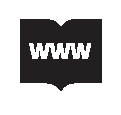
\includegraphics[height=1em]{../icons/www.eps}} Find the answers with the shortcodes:
 \par \begin{tabular}[h]{ccc}
 (1.) l2b  &  (2.) l2j  &  (3.) l4F  \end{tabular}
\end{enumerate}
}
\end{exercises}

Remember that the technique of addition and subtraction just discussed can only be applied to vectors acting along a straight line. When vectors are not in a straight line, i.e. at an angle to each other then simple geometric and trigonometric techniques can be used to find resultant vectors.

\begin{exercises}{More Resultant Vectors} \noindent
\begin{enumerate}[noitemsep, label=\textbf{\arabic*}.] 
\item A frog is trying to cross a river. It swims at 3 \ms in a northerly direction towards the opposite bank. The water is flowing in a westerly direction at 5 \ms. Find the frog's resultant velocity by using appropriate calculations. Include a rough sketch of the situation in your answer.
\item Mpihlonhle walks to the shop by walking 500 m Northwest and then 400 m N 30$^\circ$ E. Determine her resultant displacement by doing appropriate calculations.
\end{enumerate}

  \label{59e414b70efc194a27a122db47d06ce6**end}
\par \raisebox{-0.2em}{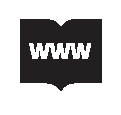
\includegraphics[height=1em]{../icons/www.eps}} Find the answers with the shortcodes:
 \par \begin{tabular}[h]{cc}
 (1.) l4L  &  (2.) lDq   & \end{tabular}
\end{exercises}
\section{Components of Vectors}
In the discussion of vector addition we saw that a number of vectors acting
together can be combined to give a single vector (the resultant). In
much the same way a single vector can be broken down into a number of vectors which when added give that original vector. These vectors which sum to the original are called {\bf components} of the original vector. The process of breaking a vector into its components is called {\bf resolving into components}.

While summing a given set of vectors gives just one answer (the
resultant), a single vector can be resolved into infinitely many sets
of components. In the diagrams below the same black vector is resolved
into different pairs of components. These components are shown as dashed lines. When added together the dashed vectors give the original black vector
(i.e. the original vector is the resultant of its components).

\begin{center}
\begin{pspicture}(-2.5,-2.6)(2.5,2.6)
%\psgrid[gridcolor=lightgray]
\psline[arrowscale=2]{->}(-2,0.5)(0,2.5)
\psline[arrowscale=2,linestyle=dashed]{->}(-2,0.5)(-2,1.25)
\psline[arrowscale=2,linestyle=dashed]{->}(-2,1.25)(0,2.5)

\psline[arrowscale=2]{->}(0.5,0.5)(2.5,2.5)
\psline[arrowscale=2,linestyle=dashed]{->}(0.5,0.5)(2.5,-0.5)
\psline[arrowscale=2,linestyle=dashed]{->}(2.5,-0.5)(2.5,2.5)
\psline[arrowscale=2]{->}(-2,-2.5)(0,-0.5)
\psline[arrowscale=2,linestyle=dashed]{->}(-2,-2.5)(0,-2.5)
\psline[arrowscale=2,linestyle=dashed]{->}(0,-2.5)(0,-0.5)
\psline{-}(-0.25,-2.25)(0,-2.25)
\psline{-}(-0.25,-2.25)(-0.25,-2.5)
\end{pspicture} 
\end{center}

In practice it is most useful to resolve a vector into components
which are at right angles to one another, usually horizontal and vertical.

Any vector can be resolved into a horizontal and a vertical component. If $\vec{A}$ is a vector, then the horizontal component of $\vec{A}$ is $\vec{A}_x$ and the vertical component is $\vec{A}_y$.

\begin{center}
\begin{pspicture}(0,-0.5)(3,3)
%\psgrid[gridcolor=lightgray]
% \psaxes[linewidth=1.2pt,labels=none,showorigin=false,ticks=none]{<->}((0,0)(-1,-1)(3,3)
\psline[arrowscale=2]{->}(0,0)(2.5,2.5)
\psline[linestyle=dashed](2.5,0)(2.5,2.5)
\psline[linestyle=dashed](0,0)(2.5,0)
\uput[ul](1,1){$\vec{A}$}
\uput[r](2.5,1.25){$\vec{A}_y$}
\uput[d](1.25,0){$\vec{A}_x$}
\psline{-}(2.25,0.25)(2.5,0.25)
\psline{-}(2.25,0)(2.25,0.25)
\psarc{->}(-1,0){1.4}{0}{15}
\rput(0.6,0.2){$\theta$}
\end{pspicture} 
\end{center}
Note that $\vec{A}_{x} = A cos \theta$ and $\vec{A}_{y} = A sin \theta$
\begin{wex}{Resolving a vector into components}{A motorist undergoes a displacement of 250~km in a direction 30$^\circ$ north of east. Resolve this displacement into components in the directions north ($\vec{x}_N$) and east ($\vec{x}_E$).\\}{
\westep{Draw a rough sketch of the original vector}
\begin{center}
\begin{pspicture}(-0.5,-0.5)(7,3.5)
%\psgrid[gridcolor=lightgray]
\psline[arrowscale=2]{->}(0,0)(6,3.46)
\pcline[offset=8pt,linestyle=none]{-}(0,0)(6,3.46)
\psarc{->}(0,0){1.4}{0}{30}
\lput{:U}{250 km}
\rput(0.9,0.25){30$^\circ$}
\psline[linestyle=dashed]{-}(0,0)(2,0)
\end{pspicture}
% \scalebox{0.7}{\pscompass}
\end{center}
\westep{Determine the vector component} 
Next we resolve the displacement into its components north and
east. Since these directions are perpendicular to one another, the
components form a right-angled triangle with the original displacement
as its hypotenuse.
\begin{center}
\begin{pspicture}(-0.5,-0.5)(7,3.5)
%\psgrid[gridcolor=lightgray]
\psline[arrowscale=2]{->}(0,0)(6,3.46)
\pcline[offset=8pt,linestyle=none]{-}(0,0)(6,3.46)
\psarc{->}(0,0){1.4}{0}{30}
\lput{:U}{250 km}
\rput(0.9,0.25){30$^\circ$}
\psline[linestyle=dashed]{-}(0,0)(2,0)
\psline[linestyle=dashed,linewidth=2pt]{->}(0,0)(6,0)
\psline[linestyle=dashed,linewidth=2pt]{->}(6,0)(6,3.46)
\pcline[offset=-8pt,linestyle=none]{-}(0,0)(6,0)
\lput{:U}{$\vec{x}_E$}
\pcline[offset=-8pt,linestyle=none]{-}(6.2,0)(6.2,3.46)
\lput{:U}{\rotateright{$\vec{x}_N$}}
\end{pspicture}
% \scalebox{0.7}{\pscompass}
\end{center}

Notice how the two components acting together give the original vector as
their resultant.

\westep{Determine the lengths of the component vectors}
Now we can use trigonometry to calculate the magnitudes of the
components of the original displacement:
\begin{eqnarray*}
x_N &=& (250) (\sin{30^\circ})\\
&=& 125\ \text{km}
\end{eqnarray*}
and
\begin{eqnarray*}
x_E &=& (250)(\cos{30^\circ})\\
&=& 216,5\ \text{km}
\end{eqnarray*}

Remember $x_N$ and $x_E$ are the magnitudes of the components -- they
are in the directions north and east respectively.}
\end{wex}

\subsection{Vector addition using components}
Components can also be used to find the resultant of vectors. This technique can be applied to both graphical and algebraic methods of finding the resultant. The method is simple: make a rough sketch of the problem, find the horizontal and vertical components of each vector, find the sum of all horizontal components and the sum of all the vertical components and then use them to find the resultant.

Consider the two vectors, $\vec{A}$ and $\vec{B}$, in Figure~\ref{fig:p:v:components:addition:vectors}, together with their resultant, $\vec{R}$. 

\begin{figure}[!htbp]
\begin{center}
\scalebox{0.7}
{
\begin{pspicture}(0,0)(8,6)%%\psgrid
%\psgrid[gridcolor=lightgray]
\psline[arrowscale=2]{->}(0,0)(5,2)
\pcline[offset=-8pt,linestyle=none](0,0)(5,2)
\lput{:U}{$\vec{A}$}
\psline[arrowscale=2]{->}(5,2)(8,6)
\pcline[offset=-8pt,linestyle=none](5,2)(8,6)
\lput{:U}{$\vec{B}$}
\psline[arrowscale=2,linewidth=2pt]{->}(0,0)(8,6)
\pcline[offset=8pt,linestyle=none](0,0)(8,6)
\lput{:U}{$\vec{R}$}
\end{pspicture}
}
\end{center}
\caption{An example of two vectors being added to give a resultant}
\label{fig:p:v:components:addition:vectors}
\end{figure}

Each vector in Figure~\ref{fig:p:v:components:addition:vectors} can be broken down into one component in the $x$-direction (horizontal) and one in the $y$-direction (vertical). These components are two vectors which when added give you the original vector as the resultant. This is shown in Figure~\ref{fig:p:v:components:addition:vectors:components} where we can see that:

\begin{minipage}{0.5\textwidth}
\begin{eqnarray*}
\vec{A}&=&\vec{A}_x+\vec{A}_y\\
\vec{B}&=&\vec{B}_x+\vec{B}_y\\
\vec{R}&=&\vec{R}_x+\vec{R}_y\\
\end{eqnarray*}
\end{minipage}
\begin{minipage}{0.5\textwidth}
\begin{eqnarray*}
\mbox{But,}\quad \vec{R}_x&=&\vec{A}_x+\vec{B}_x\\
\mbox{and}\quad\vec{R}_y&=&\vec{A}_y+\vec{B}_y\\
\end{eqnarray*}
\end{minipage}

In summary, addition of the $x$ components of the two original
vectors gives the $x$ component of the resultant. The same applies to
the $y$ components. So if we just added all the components 
together we would get the same answer! This is another important
property of vectors. 

\begin{figure}[H]
\begin{center}
\scalebox{1}
{
\begin{pspicture}(-1,-0.6)(8.6,7)
%\psgrid[gridcolor=lightgray]
%A
\psline[arrowscale=2]{->}(0,0)(5,2)
\pcline[offset=-8pt,linestyle=none](0,0)(5,2)
\lput{:U}{$\vec{A}$}
\psline[linestyle=dashed,arrowscale=2]{->}(0,0)(5,0)(5,2)	%components of A
\pcline[offset=-8pt,linestyle=none](0,0)(5,0)
\lput{:U}{$\vec{A}_x$}
\psline[linestyle=dashed,arrowscale=2]{->}(0,6.5)(5,6.5)
\pcline[offset=8pt,linestyle=none](0,6.5)(5,6.5)
\lput{:U}{$\vec{A}_x$}
\pcline[offset=-8pt,linestyle=none](5,0)(5,2)
\lput{:U}{$\vec{A}_y$}
\psline[linestyle=dashed,arrowscale=2]{->}(-0.5,0)(-0.5,2)
\pcline[offset=8pt,linestyle=none](-0.5,0)(-0.5,2)
\lput{:U}{$\vec{A}_y$}
%Right angle in corner! (5,0)
\psline[linestyle=dashed,arrowscale=2](4.7,0)(4.7,0.3)
\psline[linestyle=dashed,arrowscale=2](4.7,0.3)(5.,0.3)
%B
\psline[arrowscale=2]{->}(5,2)(8,6)
\pcline[offset=-8pt,linestyle=none](5,2)(8,6)
\lput{:U}{$\vec{B}$}
\psline[linestyle=dashed,arrowscale=2]{->}(5,2)(8,2)(8,6)	%components of B
\pcline[offset=-8pt,linestyle=none](5,2)(8,2)
\lput{:U}{$\vec{B}_x$}
\psline[linestyle=dashed,arrowscale=2]{->}(5,6.5)(8,6.5)
\pcline[offset=8pt,linestyle=none](5,6.5)(8,6.5)
\lput{:U}{$\vec{B}_x$}
\pcline[offset=-8pt,linestyle=none](8,2)(8,6)
\lput{:U}{$\vec{B}_y$}
\psline[linestyle=dashed,arrowscale=2]{->}(-0.5,2)(-0.5,6)
\pcline[offset=8pt,linestyle=none](-0.5,2)(-0.5,6)
\lput{:U}{$\vec{B}_y$}
%Right angle in corner (8,2)
\psline[linestyle=dashed,arrowscale=2](7.7,2)(7.7,2.3)
\psline[linestyle=dashed,arrowscale=2](7.7,2.3)(8,2.3)
%R
\psline[arrowscale=2,linewidth=2pt]{->}(0,0)(8,6)
\pcline[offset=8pt,linestyle=none](0,0)(8,6)
\lput{:U}{$\vec{R}$}
\psline[linestyle=dashed,arrowscale=2]{->}(0,0)(0,6)(8,6)	%components of B
\pcline[offset=-8pt,linestyle=none](0,6)(8,6)
\lput{:U}{$\vec{R}_x$}
\pcline[offset=-8pt,linestyle=none](0,0)(0,6)
\lput{:U}{$\vec{R}_y$}
%Right angle in corner (0,6)
\psline[linestyle=dashed,arrowscale=2](0,5.7)(0.3,5.7)
\psline[linestyle=dashed,arrowscale=2](0.3,5.7)(0.3,6)
\end{pspicture}
}
\end{center}
\caption{Adding vectors using components.}
\label{fig:p:v:components:addition:vectors:components}
\end{figure}
To find the resultant we note that $R=\sqrt{R_{x}^{2} + R_{y}^{2}}$. To find the angle we use $\theta = tan^{-1} (\frac{R_{y}}{R_{x}})$.
\begin{wex}{Adding Vectors Using Components}{If in Figure~\ref{fig:p:v:components:addition:vectors:components}, $\vec{A}=5,385\emm$ at an angle of 21.8$^\circ$ to the horizontal and $\vec{B}=5\emm$ at an angle of 53,13$^\circ$ to the horizontal, find $\vec{R}$.\\}{
\westep{Decide how to tackle the problem} 
The first thing we must realise is that the order that we add the vectors does not matter. Therefore, we can work through the vectors to be added in any order.

\westep{Resolve $\vec{A}$ into components}
We find the components of $\vec{A}$ by using known trigonometric ratios. First we find the magnitude of the vertical component, $A_y$:
\begin{eqnarray*}
\sin \theta &=& \frac{A_y}{A} \\
\sin{21,8^\circ} &=& \frac{A_y}{5,385}\\
A_y &=& (5,385)(\sin{21,8^\circ})\\
 &=& 2\emm
\end{eqnarray*}

Secondly we find the magnitude of the horizontal component, $A_x$:
\begin{eqnarray*}
\cos \theta &=& \frac{A_x}{A} \\
\cos{21.8^\circ} &=& \frac{A_x}{5,385}\\
A_x &=& (5,385) (\cos{21,8^\circ})\\
 &=& 5\emm
\end{eqnarray*}

\begin{center}
\begin{pspicture}(-0.2,-0.6)(5.6,2.4)%%\psgrid
%\psgrid[gridcolor=lightgray]
\psline[arrowscale=2]{->}(0,0)(5,2)
\pcline[offset=8pt]{|-|}(0,0)(5,2)
\lput*{:U}{5,385 m}
\psline[linestyle=dashed,arrowscale=2]{->}(0,0)(5,0)
\pcline[offset=-8pt]{|-|}(0,0)(5,0)
\lput*{:U}{5 m}
\psline[linestyle=dashed,arrowscale=2]{->}(5,0)(5,2)
\pcline[offset=-8pt]{|-|}(5,0)(5,2)
\lput*{:U}{2 m}
%Right angle in corner! (5,0)
\psline[linestyle=dashed,arrowscale=2](4.7,0)(4.7,0.3)
\psline[linestyle=dashed,arrowscale=2](4.7,0.3)(5.,0.3)
\end{pspicture}
\end{center}

The components give the sides of the right angle triangle, for which the original vector, $\vec{A}$, is the hypotenuse. 

\westep{Resolve $\vec{B}$ into components}
We find the components of $\vec{B}$ by using known trigonometric ratios. First we find the magnitude of the vertical component, $B_y$:
\begin{eqnarray*}
\sin{\theta} & = & \frac{B_y}{B} \\
\sin{53,13^\circ} & = &\frac{B_y}{5}\\
B_y & = & (5)(\sin{53,13^\circ})\\
 & = & 4\emm
\end{eqnarray*}

Secondly we find the magnitude of the horizontal component, $B_x$:
\begin{eqnarray*}
\cos{\theta} &=& \frac{B_x}{B} \\
\cos{21,8^\circ} &=& \frac{B_x}{5,385}\\
B_x & = & (5,385) (\cos{53,13^\circ})\\
& = & 5\emm
\end{eqnarray*}

\begin{center}
\begin{pspicture}(4.6,1.4)(8.6,6.4)
%\psgrid[gridcolor=lightgray]
\psline[arrowscale=2]{->}(5,2)(8,6)
\pcline[offset=8pt]{|-|}(5,2)(8,6)
\lput*{:U}{5 m}
\psline[linestyle=dashed,arrowscale=2]{->}(5,2)(8,2)
\pcline[offset=-8pt]{|-|}(5,2)(8,2)
\lput*{:U}{3 m}
\psline[linestyle=dashed,arrowscale=2]{->}(8,2)(8,6)
\pcline[offset=-8pt]{|-|}(8,2)(8,6)
\lput*{:U}{4 m}
%Right angle in corner (8,2)
\psline[linestyle=dashed,arrowscale=2](7.7,2)(7.7,2.3)
\psline[linestyle=dashed,arrowscale=2](7.7,2.3)(8,2.3)
\end{pspicture}
\end{center}

\westep{Determine the components of the resultant vector}
Now we have all the components. If we add all the horizontal components then
we will have the $x$-component of the resultant vector, $\vec{R}_x$.  Similarly, we add all the vertical components then we will have the $y$-component of the resultant vector, $\vec{R}_y$.
\begin{eqnarray*}
R_x &=& A_x+B_x\\
&=&5\emm + 3\emm\\
&=&8\emm
\end{eqnarray*}
Therefore, $\vec{R}_x$ is 8 m to the right.
\begin{eqnarray*}
R_y &=& A_y+B_y\\
&=&2\emm + 4\emm\\
&=&6\emm
\end{eqnarray*}
Therefore, $\vec{R}_y$ is 6 m up.

\westep{Determine the magnitude and direction of the resultant vector}
Now that we have the components of the resultant, we can use the Theorem of Pythagoras to determine the magnitude of the resultant, $R$.
\begin{eqnarray*}
R^2&=&(R_x)^2 + (R_y)^2\\
R^2&=&(6)^2 + (8)^2\\
R^2&=&100\\
\therefore R&=&10\emm
\end{eqnarray*}

\begin{center}
\begin{pspicture}(-1,-0.4)(8.4,7)
%\psgrid[gridcolor=lightgray]
\psline[arrowscale=2]{->}(0,0)(8,6)
\pcline[offset=-8pt]{|-|}(0,0)(8,6)
\lput*{:U}{10 m}

\psline[linestyle=dashed,arrowscale=2]{->}(0,0)(0,6)
\psline[linestyle=dashed,arrowscale=2]{->}(-.5,0)(-0.5,2)
\psline[linestyle=dashed,arrowscale=2]{->}(-0.5,2)(-0.5,6)
\pcline[offset=8pt]{|-|}(-.5,0)(-0.5,6)
\lput*{:U}{6 m}

\psline[linestyle=dashed,arrowscale=2]{->}(0,6)(8,6)
\psline[linestyle=dashed,arrowscale=2]{->}(0,6.5)(5,6.5)
\psline[linestyle=dashed,arrowscale=2]{->}(5,6.5)(8,6.5)
\pcline[offset=8pt]{|-|}(0,6.5)(8,6.5)
\lput*{:U}{8 m} 

%Right angle in corner (0,6)
\psline[linestyle=dashed,arrowscale=2](0,5.7)(0.3,5.7)
\psline[linestyle=dashed,arrowscale=2](0.3,5.7)(0.3,6)
\psline[linestyle=dashed,arrowscale=2](0,0)(4,0)
\rput(0.7,0.25){$\alpha$}
\psarc{->}(0,0){1}{0}{36.8}
\end{pspicture}
\end{center}

The magnitude of the resultant, $R$ is 10 m.  So all we have to do is calculate its direction. We can specify the direction as the angle the vectors makes with a known direction. To do this you only need to visualise the vector as starting at the origin of a coordinate system. We have drawn this explicitly below and the angle we will calculate is labeled $\alpha$.

Using our known trigonometric ratios we can calculate the value of $\alpha$;
\begin{eqnarray*}
\tan \alpha & = & \frac{6 \emm}{8\emm} \\
\alpha & = & \tan^{-1} \frac{6\emm}{8\emm}\\
\alpha & = & 36,8^o.
\end{eqnarray*}
\westep{Quote the final answer}
$\vec{R}$ is 10 m at an angle of $36,8^\circ$ to the positive $x$-axis.}
\end{wex}

\begin{exercises}{Adding and Subtracting Components of Vectors}{
\begin{enumerate}[noitemsep, label=\textbf{\arabic*}.]
\item Harold walks to school by walking 600 m Northeast and then 500 m N $40^o$ W. Determine his resultant displacement by means of addition of components of vectors.
\item A dove flies from her nest, looking for food for her chick. She flies at a velocity of 2 \ms on a bearing of 135${^o}$ in a wind with a velocity of 1,2 \ms on a bearing of 230${^o}$. Calculate her resultant velocity by adding the horizontal and vertical components of vectors.
\end{enumerate}
}
\par \raisebox{-0.2em}{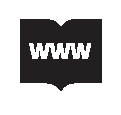
\includegraphics[height=1em]{../icons/www.eps}} Find the answers with the shortcodes:
 \par \begin{tabular}[h]{cc}
 (1.) l4e  &  (2.) l2Z   & \end{tabular}
\end{exercises}

\subsection*{Summary}
\begin{itemize}
\item A scalar is a physical quantity with magnitude only.
\item A vector is a physical quantity with magnitude and direction.
\item Vectors may be represented as arrows where the length of the arrow indicates the magnitude and the arrowhead indicates the direction of the vector.
\item The direction of a vector can be indicated by referring to another vector or a fixed point (eg. $30^{\circ}$ from the river bank); using a compass (eg. N $30^\circ$ W); or bearing (eg. $053 ^\circ$).
\end{itemize}
\begin{eocexercises}{Vectors}\noindent
\begin{enumerate}[noitemsep, label=\textbf{\arabic*}.]
          \label{m38819*uid92}\item A point is acted on by two forces in equilibrium. The forces
\label{m38819*id197705}\begin{enumerate}[noitemsep, label=\textbf{\alph*}. ] 
            \label{m38819*uid93}\item have equal magnitudes and directions.
\label{m38819*uid94}\item have equal magnitudes but opposite directions.
\label{m38819*uid95}\item act perpendicular to each other.
\label{m38819*uid96}\item act in the same direction.
\end{enumerate}
                \label{m38819*uid97}\item A point in equilibrium is acted on by three forces. Force ${F}_{1}$ has components $15 ~\text{N}$ due south and $13 ~\text{N}$ due west. What are the components of force ${F}_{2}$?
\label{m38819*id197809}\begin{enumerate}[noitemsep, label=\textbf{\alph*}. ] 
            \label{m38819*uid98}\item 13 N due north and $20 ~\text{N}$ due west
\label{m38819*uid99}\item $13 ~\text{N}$ due north and $13 ~\text{N}$ due west
\label{m38819*uid100}\item $15 ~\text{N}$due north and $7 ~\text{N}$ due west
\label{m38819*uid101}\item $15 ~\text{N}$ due north and $13 ~\text{N}$ due east
\end{enumerate}
    \setcounter{subfigure}{0}
	\begin{figure}[H] % horizontal\label{m38819*id197871}
    \begin{center}
\begin{pspicture}(-0.5,-2.0085938)(4.005625,2.0085938) \psline[linewidth=0.04cm,linestyle=dashed,dash=0.16cm 0.16cm](1.9996876,1.7373438)(1.9996876,-1.6626563) \psline[linewidth=0.04cm,linestyle=dashed,dash=0.16cm 0.16cm](0.2996875,0.03734375)(3.6996875,0.03734375) \psline[linewidth=0.04cm,arrowsize=0.0529cm 3.17,arrowlength=1.4,arrowinset=0.0]{->}(1.9996876,0.03734375)(3.2996874,0.03734375) \psline[linewidth=0.04cm,arrowsize=0.05291667cm 3.17,arrowlength=1.4,arrowinset=0.0]{->}(1.9996876,0.03734375)(0.8996875,1.6373438) \psline[linewidth=0.04cm,arrowsize=0.05291667cm 3.17,arrowlength=1.4,arrowinset=0.0]{->}(1.9996876,0.03734375)(0.6996875,-1.2626562) \usefont{T1}{ptm}{m}{n} \rput(1.9879688,1.8373437){\footnotesize N} \usefont{T1}{ptm}{m}{n} \rput(0.13625,0.03734375){\footnotesize W} \usefont{T1}{ptm}{m}{n} \rput(1.9701562,-1.8626562){\footnotesize S} \usefont{T1}{ptm}{m}{n} \rput(3.8676562,0.03734375){\footnotesize E} \usefont{T1}{ptm}{m}{n} \rput(2.5396874,-0.16265625){\footnotesize 20 N} \usefont{T1}{ptm}{m}{n} \rput(1.5371875,1.1373438){\footnotesize F$_2$} \usefont{T1}{ptm}{m}{n} \rput(1.5371875,-0.86265624){\footnotesize F$_1$}
\end{pspicture} 
    \end{center}
 \end{figure}               \label{m38819*uid102}\item Which of the following contains two vectors and a scalar?
\label{m38819*id197890}\begin{enumerate}[noitemsep, label=\textbf{\alph*}. ] 
            \label{m38819*uid103}\item distance, acceleration, speed
\label{m38819*uid104}\item displacement, velocity, acceleration
\label{m38819*uid105}\item distance, mass, speed
\label{m38819*uid106}\item displacement, speed, velocity
\end{enumerate}
                \label{m38819*uid107}\item Two vectors act on the same point. What should the angle between them be so that a maximum resultant is obtained?
\label{m38819*id197965}\begin{enumerate}[noitemsep, label=\textbf{\alph*}. ] 
            \label{m38819*uid108}\item $0{}^{\circ }$\label{m38819*uid109}\item $90{}^{\circ }$\label{m38819*uid110}\item $180{}^{\circ }$\label{m38819*uid111}\item cannot tell
\end{enumerate}
                \label{m38819*uid112}\item Two forces, $4 ~\text{N}$ and $11 ~\text{N}$, act on a point. Which one of the following \uline{cannot} be the magnitude of a resultant?
\label{m38819*id198082}\begin{enumerate}[noitemsep, label=\textbf{\alph*}. ] 
            \label{m38819*uid113}\item $4 ~\text{N}$
\label{m38819*uid114}\item $7 ~\text{N}$
\label{m38819*uid115}\item $11 ~\text{N}$
\label{m38819*uid116}\item $15 ~\text{N}$
\end{enumerate}

            \label{m38819*uid118}\item A helicopter flies due east with an air speed of $150\phantom{\rule{2pt}{0ex}}\text{km}\ensuremath{\cdot}\text{h}{}^{-1}$. It flies through an air current which moves at $200\phantom{\rule{2pt}{0ex}}\text{km}\ensuremath{\cdot}\text{h}{}^{-1}$ north. Given this information, answer the following questions:
\label{m38819*id198203}\begin{enumerate}[noitemsep, label=\textbf{\alph*}. ] 
            \label{m38819*uid119}\item In which direction does the helicopter fly?
% \label{m38819*uid120}\item What is the ground speed of the helicopter?
% \label{m38819*uid121}\item Calculate the ground distance covered in 40 minutes by the helicopter.
\end{enumerate}
                \label{m38819*uid122}\item A plane must fly 70 km due north. A cross wind is blowing to the west at $30\phantom{\rule{2pt}{0ex}}\text{km}\ensuremath{\cdot}\text{h}{}^{-1}$. In which direction must the pilot steer if the plane flies at a speed of $200\phantom{\rule{2pt}{0ex}}\text{km}\ensuremath{\cdot}\text{h}{}^{-1}$ in windless conditions?\newline
\label{m38819*uid123}\item A stream that is 280 m wide flows along its banks with a velocity of $1,80\phantom{\rule{2pt}{0ex}}\text{m}\ensuremath{\cdot}\text{s}{}^{-1}$. A raft can travel at a speed of $2,50\phantom{\rule{2pt}{0ex}}\text{m}\ensuremath{\cdot}\text{s}{}^{-1}$ across the stream. Answer the following questions:
\label{m38819*id198337}\begin{enumerate}[noitemsep, label=\textbf{\alph*}. ] 
%             \label{m38819*uid124}\item What is the shortest time in which the raft can cross the stream?
% \label{m38819*uid125}\item How far does the raft drift downstream in that time?
\label{m38819*uid126}\item In what direction must the raft be steered against the current so that it crosses the stream perpendicular to its banks?
% \label{m38819*uid127}\item How long does it take to cross the stream in part c?
\end{enumerate}
                \label{m38819*uid128}\item A helicopter is flying from place $X$ to place $Y$. $Y$ is 1 000~km away in a direction ${50}^{\circ }$ east of north and the pilot wishes to reach it in two hours. There is a wind of speed $150\phantom{\rule{2pt}{0ex}}\text{km}\ensuremath{\cdot}\text{h}{}^{-1}$ blowing from the northwest. Find, by accurate construction and measurement (with a scale of $1\phantom{\rule{3.33333pt}{0ex}}\text{cm}=50\phantom{\rule{3.33333pt}{0ex}}{\text{km}\ensuremath{\cdot}\text{h}}^{-1}$), the
\label{m38819*id198505}\begin{enumerate}[noitemsep, label=\textbf{\alph*}. ] 
            \label{m38819*uid129}\item direction in which the helicopter must fly
% \label{m38819*uid130}\item magnitude of the velocity required for it to reach its destination on time.
\end{enumerate}
                \label{m38819*uid131}\item An aeroplane is flying towards a destination 300~km due south from its present position. There is a wind blowing from the north east at $120\phantom{\rule{2pt}{0ex}}\text{km}\ensuremath{\cdot}\text{h}{}^{-1}$. The aeroplane needs to reach its destination in 30 minutes. Find, by accurate construction and measurement (with a scale of $1\phantom{\rule{3.33333pt}{0ex}}\text{cm}=30\phantom{\rule{3.33333pt}{0ex}}{\text{km}\ensuremath{\cdot}\text{s}}^{-1}$), or otherwise,
\label{m38819*id198608}\begin{enumerate}[noitemsep, label=\textbf{\alph*}. ] 
            \label{m38819*uid132}\item the direction in which the aeroplane must fly and
% \label{m38819*uid133}\item the speed which the aeroplane must maintain in order to reach the destination on time.
\label{m38819*uid134}\item Confirm your answers in the previous 2 sub-questions with calculations.
\end{enumerate}
                \label{m38819*uid135}\item An object of weight $W$ is supported by two cables attached to the ceiling and wall as shown. The tensions in the two cables are ${T}_{1}$ and ${T}_{2}$ respectively. Tension ${T}_{1}=1200\phantom{\rule{2pt}{0ex}}\text{N}$. Determine the tension ${T}_{2}$ and weight $W$ of the object by accurate construction and measurement or by calculation.
    \setcounter{subfigure}{0}
	\begin{figure}[H] % horizontal\label{m38819*id198746}
    \begin{center}
\begin{pspicture}(0,-2.03)(6.4809375,2.03) \psline[linewidth=0.04cm](0.4809375,2.01)(0.4809375,-2.01) \psline[linewidth=0.04cm](0.4809375,2.01)(6.4609375,2.01) \psframe[linewidth=0.04,dimen=outer](3.9409375,-1.3730845)(3.0009375,-1.9700994) \psline[linewidth=0.04cm](3.4809375,-0.77606964)(3.4809375,-1.3929851) \psline[linewidth=0.04cm,arrowsize=0.05291667cm 2.0,arrowlength=1.4,arrowinset=0.4]{->}(3.4809375,-0.79597014)(5.5809374,2.01) \psline[linewidth=0.04cm,arrowsize=0.05291667cm 2.0,arrowlength=1.4,arrowinset=0.4]{->}(3.4809375,-0.79)(0.5009375,0.27) \usefont{T1}{ptm}{m}{n} \rput(4.872031,0.5){T$_1$} 
\usefont{T1}{ptm}{m}{n} \rput(1.7120312,-0.44){T$_2$} 
\usefont{T1}{ptm}{m}{n} \rput(3.4745312,-1.68){W} 
\usefont{T1}{ptm}{m}{n} \rput(5.114375,1.78){45$^\circ$} 
\usefont{T1}{ptm}{m}{n} \rput(0.8640625,-0.14){70$^\circ$} 
\end{pspicture}
    \end{center}
 \end{figure}   
            \label{m38819*uid136}\item In a map-work exercise, hikers are required to walk from a tree marked A on the map to another tree marked B which lies 2,0 km due East of A. The hikers then walk in a straight line to a waterfall in position C which has components measured from B of 1,0 km E and 4,0 km N.
\label{m38819*id198765}\begin{enumerate}[noitemsep, label=\textbf{\alph*}. ] 
            \label{m38819*uid137}\item Distinguish between quantities that are described as being \textsl{vector} and \textsl{scalar}.
\label{m38819*uid138}\item Draw a labeled displacement-vector diagram (not necessarily to scale) of the hikers' complete journey.
\label{m38819*uid139}\item What is the total distance walked by the hikers from their starting point at A to the waterfall C?
\label{m38819*uid140}\item What are the magnitude and bearing, to the nearest degree, of the displacement of the hikers from their starting point to the waterfall?
\end{enumerate}
                \label{m38819*uid141}\item An object $X$ is supported by two strings, $A$ and $B$, attached to the ceiling as shown in the sketch. Each of these strings can withstand a maximum force of 700~N. The weight of $X$ is increased gradually.
\label{m38819*id198883}\begin{enumerate}[noitemsep, label=\textbf{\alph*}. ] 
            \label{m38819*uid142}\item Draw a rough sketch of the triangle of forces, and use it to explain which string will break first.
\label{m38819*uid143}\item Determine the maximum weight of $X$ which can be supported.
\end{enumerate}
    \setcounter{subfigure}{0}
	\begin{figure}[H] % horizontal\label{m38819*id198922}
\begin{center}
 \scalebox{0.75} % Change this value to rescale the drawing.
{
\begin{pspicture}(-0.5,-1.8014708)(6.04,1.8385292)
\psline[linewidth=0.08cm](0.0,1.7985293)(6.0,1.7985293)
\psframe[linewidth=0.04,dimen=outer](4.0,-0.80147076)(3.0,-1.8014708)
\psline[linewidth=0.04cm](0.8,1.7985293)(3.5,0.09852926)
\psline[linewidth=0.04cm](5.297232,1.8014708)(3.5,0.09852926)
\psline[linewidth=0.04cm](3.5,-0.80147076)(3.5,0.09852926)
\psline[linewidth=0.04cm](4.0,-0.101470746)(4.0,-0.101470746)
\usefont{T1}{ptm}{m}{n}
\rput(3.5265625,-1.2914708){$X$}
\usefont{T1}{ptm}{m}{n}
\rput(1.8265625,0.50852925){$A$}
\usefont{T1}{ptm}{m}{n}
\rput(5.0071874,0.70852923){$B$}
\usefont{T1}{ptm}{m}{n}
\rput(4.4335938,1.4085293){45$^\circ$}
\usefont{T1}{ptm}{m}{n}
\rput(2.038125,1.4085293){30$^\circ$}
\end{pspicture} 
}
\end{center}
 \end{figure}  
             \label{m38819*uid144}\item A rope is tied at two points which are 70~cm apart from each other, on the same horizontal line. The total length of rope is 1~m, and the maximum tension it can withstand in any part is 1000~N. Find the largest mass ($m$), in kg, that can be carried at the midpoint of the rope, without breaking the rope. Include a vector diagram in your answer.
    \setcounter{subfigure}{0}
	\begin{figure}[H] % horizontal\label{m38819*id198958}
    \begin{center}
\scalebox{0.75} % Change this value to rescale the drawing.
{
\begin{pspicture}(0,-1.098125)(9.04,1.098125)
\psline[linewidth=0.08cm](0.0,0.941875)(2.0,0.941875)
\psline[linewidth=0.08cm](2.0,0.941875)(2.0,-1.058125)
\psline[linewidth=0.08cm](7.0,0.941875)(7.0,-1.058125)
\psline[linewidth=0.08cm](7.0,0.941875)(9.0,0.941875)
\psframe[linewidth=0.04,dimen=outer](5.1,-0.058125)(3.9,-0.758125)
\psline[linewidth=0.024cm](2.0,0.941875)(4.5,-0.058125)
\psline[linewidth=0.024cm](4.5,-0.058125)(7.0,0.941875)
\psline[linewidth=0.03cm,linestyle=dashed,dash=0.16cm 0.16cm,arrowsize=0.05291667cm 2.0,arrowlength=1.4,arrowinset=0.4]{<->}(2.0,0.941875)(7.0,0.941875)
\usefont{T1}{ptm}{m}{n}
\rput(4.5376563,-0.448125){$m$}
\usefont{T1}{ptm}{m}{n}
\rput(4.5878124,0.936875){\footnotesize \psframebox*[framesep=0, boxsep=false,fillcolor=white] {70 cm}}
\end{pspicture} 
}
    \end{center}
 \end{figure}               \end{enumerate}
  \label{m38819**end}
  \label{59e414b70efc194a27a122db47d06ce6**end}
\par \raisebox{-0.2em}{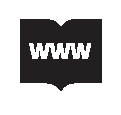
\includegraphics[height=1em]{../icons/www.eps}} Find the answers with the shortcodes:
 \par \begin{tabular}[h]{cccccc}
 (1.) l20  &  (2.) l28  &  (3.) l29  &  (4.) l2X  &  (5.) l2I  &  (6.) l25  &  (7.) l2N  &  (8.) l2R  &  (9.) l2n  & 
(10.) l2E & (11.) l2m & (12.) l2y & (13.) l2V & (14.) l2p 
\end{tabular}
\end{eocexercises}
